\documentclass[twoside]{book}

% Packages required by doxygen
\usepackage{fixltx2e}
\usepackage{calc}
\usepackage{doxygen}
\usepackage[export]{adjustbox} % also loads graphicx
\usepackage{graphicx}
\usepackage[utf8]{inputenc}
\usepackage{makeidx}
\usepackage{multicol}
\usepackage{multirow}
\PassOptionsToPackage{warn}{textcomp}
\usepackage{textcomp}
\usepackage[nointegrals]{wasysym}
\usepackage[table]{xcolor}

% Font selection
\usepackage[T1]{fontenc}
\usepackage[scaled=.90]{helvet}
\usepackage{courier}
\usepackage{amssymb}
\usepackage{sectsty}
\renewcommand{\familydefault}{\sfdefault}
\allsectionsfont{%
  \fontseries{bc}\selectfont%
  \color{darkgray}%
}
\renewcommand{\DoxyLabelFont}{%
  \fontseries{bc}\selectfont%
  \color{darkgray}%
}
\newcommand{\+}{\discretionary{\mbox{\scriptsize$\hookleftarrow$}}{}{}}

% Page & text layout
\usepackage{geometry}
\geometry{%
  a4paper,%
  top=2.5cm,%
  bottom=2.5cm,%
  left=2.5cm,%
  right=2.5cm%
}
\tolerance=750
\hfuzz=15pt
\hbadness=750
\setlength{\emergencystretch}{15pt}
\setlength{\parindent}{0cm}
\setlength{\parskip}{3ex plus 2ex minus 2ex}
\makeatletter
\renewcommand{\paragraph}{%
  \@startsection{paragraph}{4}{0ex}{-1.0ex}{1.0ex}{%
    \normalfont\normalsize\bfseries\SS@parafont%
  }%
}
\renewcommand{\subparagraph}{%
  \@startsection{subparagraph}{5}{0ex}{-1.0ex}{1.0ex}{%
    \normalfont\normalsize\bfseries\SS@subparafont%
  }%
}
\makeatother

% Headers & footers
\usepackage{fancyhdr}
\pagestyle{fancyplain}
\fancyhead[LE]{\fancyplain{}{\bfseries\thepage}}
\fancyhead[CE]{\fancyplain{}{}}
\fancyhead[RE]{\fancyplain{}{\bfseries\leftmark}}
\fancyhead[LO]{\fancyplain{}{\bfseries\rightmark}}
\fancyhead[CO]{\fancyplain{}{}}
\fancyhead[RO]{\fancyplain{}{\bfseries\thepage}}
\fancyfoot[LE]{\fancyplain{}{}}
\fancyfoot[CE]{\fancyplain{}{}}
\fancyfoot[RE]{\fancyplain{}{\bfseries\scriptsize Generated by Doxygen }}
\fancyfoot[LO]{\fancyplain{}{\bfseries\scriptsize Generated by Doxygen }}
\fancyfoot[CO]{\fancyplain{}{}}
\fancyfoot[RO]{\fancyplain{}{}}
\renewcommand{\footrulewidth}{0.4pt}
\renewcommand{\chaptermark}[1]{%
  \markboth{#1}{}%
}
\renewcommand{\sectionmark}[1]{%
  \markright{\thesection\ #1}%
}

% Indices & bibliography
\usepackage{natbib}
\usepackage[titles]{tocloft}
\setcounter{tocdepth}{3}
\setcounter{secnumdepth}{5}
\makeindex

% Hyperlinks (required, but should be loaded last)
\usepackage{ifpdf}
\ifpdf
  \usepackage[pdftex,pagebackref=true]{hyperref}
\else
  \usepackage[ps2pdf,pagebackref=true]{hyperref}
\fi
\hypersetup{%
  colorlinks=true,%
  linkcolor=blue,%
  citecolor=blue,%
  unicode%
}

% Custom commands
\newcommand{\clearemptydoublepage}{%
  \newpage{\pagestyle{empty}\cleardoublepage}%
}

\usepackage{caption}
\captionsetup{labelsep=space,justification=centering,font={bf},singlelinecheck=off,skip=4pt,position=top}

%===== C O N T E N T S =====

\begin{document}

% Titlepage & ToC
\hypersetup{pageanchor=false,
             bookmarksnumbered=true,
             pdfencoding=unicode
            }
\pagenumbering{alph}
\begin{titlepage}
\vspace*{7cm}
\begin{center}%
{\Large Pet\+Fera }\\
\vspace*{1cm}
{\large Generated by Doxygen 1.8.14}\\
\end{center}
\end{titlepage}
\clearemptydoublepage
\pagenumbering{roman}
\tableofcontents
\clearemptydoublepage
\pagenumbering{arabic}
\hypersetup{pageanchor=true}

%--- Begin generated contents ---
\chapter{Hierarchical Index}
\section{Class Hierarchy}
This inheritance list is sorted roughly, but not completely, alphabetically\+:\begin{DoxyCompactList}
\item \contentsline{section}{Animal}{\pageref{class_animal}}{}
\begin{DoxyCompactList}
\item \contentsline{section}{Anfibio}{\pageref{class_anfibio}}{}
\begin{DoxyCompactList}
\item \contentsline{section}{Mamifero}{\pageref{class_mamifero}}{}
\begin{DoxyCompactList}
\item \contentsline{section}{Reptil}{\pageref{class_reptil}}{}
\begin{DoxyCompactList}
\item \contentsline{section}{Ave}{\pageref{class_ave}}{}
\end{DoxyCompactList}
\end{DoxyCompactList}
\end{DoxyCompactList}
\end{DoxyCompactList}
\item \contentsline{section}{funcionario}{\pageref{classfuncionario}}{}
\begin{DoxyCompactList}
\item \contentsline{section}{Veterinario}{\pageref{class_veterinario}}{}
\end{DoxyCompactList}
\item invalid\+\_\+argument\begin{DoxyCompactList}
\item \contentsline{section}{Erro\+Animal}{\pageref{class_erro_animal}}{}
\item \contentsline{section}{Erro\+De\+Insercao}{\pageref{class_erro_de_insercao}}{}
\item \contentsline{section}{Erro\+Funcionario}{\pageref{class_erro_funcionario}}{}
\item \contentsline{section}{Erro\+Id}{\pageref{class_erro_id}}{}
\item \contentsline{section}{Erro\+Tipo\+Sanguineo}{\pageref{class_erro_tipo_sanguineo}}{}
\end{DoxyCompactList}
\end{DoxyCompactList}

\chapter{Class Index}
\section{Class List}
Here are the classes, structs, unions and interfaces with brief descriptions\+:\begin{DoxyCompactList}
\item\contentsline{section}{\mbox{\hyperlink{class_anfibio}{Anfibio}} \\*Criação da classe \mbox{\hyperlink{class_anfibio}{Anfibio}} }{\pageref{class_anfibio}}{}
\item\contentsline{section}{\mbox{\hyperlink{class_animal}{Animal}} \\*Criação da classe \mbox{\hyperlink{class_animal}{Animal}} }{\pageref{class_animal}}{}
\item\contentsline{section}{\mbox{\hyperlink{class_ave}{Ave}} \\*Criação da classe \mbox{\hyperlink{class_ave}{Ave}} }{\pageref{class_ave}}{}
\item\contentsline{section}{\mbox{\hyperlink{class_erro_animal}{Erro\+Animal}} \\*Um tratamento de excessão }{\pageref{class_erro_animal}}{}
\item\contentsline{section}{\mbox{\hyperlink{class_erro_de_insercao}{Erro\+De\+Insercao}} \\*Um tratamento de excessão }{\pageref{class_erro_de_insercao}}{}
\item\contentsline{section}{\mbox{\hyperlink{class_erro_funcionario}{Erro\+Funcionario}} \\*Um tratamento de excessão }{\pageref{class_erro_funcionario}}{}
\item\contentsline{section}{\mbox{\hyperlink{class_erro_id}{Erro\+Id}} \\*Um tratamento de excessão }{\pageref{class_erro_id}}{}
\item\contentsline{section}{\mbox{\hyperlink{class_erro_tipo_sanguineo}{Erro\+Tipo\+Sanguineo}} \\*Um tratamento de excessão }{\pageref{class_erro_tipo_sanguineo}}{}
\item\contentsline{section}{\mbox{\hyperlink{classfuncionario}{funcionario}} \\*Criação da classe funcionário }{\pageref{classfuncionario}}{}
\item\contentsline{section}{\mbox{\hyperlink{class_mamifero}{Mamifero}} \\*Criação da classe \mbox{\hyperlink{class_mamifero}{Mamifero}} }{\pageref{class_mamifero}}{}
\item\contentsline{section}{\mbox{\hyperlink{class_reptil}{Reptil}} \\*Criação da classe \mbox{\hyperlink{class_reptil}{Reptil}} }{\pageref{class_reptil}}{}
\item\contentsline{section}{\mbox{\hyperlink{class_veterinario}{Veterinario}} \\*Criação da classe \mbox{\hyperlink{class_veterinario}{Veterinario}} }{\pageref{class_veterinario}}{}
\end{DoxyCompactList}

\chapter{File Index}
\section{File List}
Here is a list of all documented files with brief descriptions\+:\begin{DoxyCompactList}
\item\contentsline{section}{doxygen/{\bfseries anfibio.\+h} }{\pageref{anfibio_8h}}{}
\item\contentsline{section}{doxygen/{\bfseries animal.\+h} }{\pageref{animal_8h}}{}
\item\contentsline{section}{doxygen/{\bfseries ave.\+h} }{\pageref{ave_8h}}{}
\item\contentsline{section}{doxygen/{\bfseries funcionario.\+h} }{\pageref{funcionario_8h}}{}
\item\contentsline{section}{doxygen/\mbox{\hyperlink{main_8cpp}{main.\+cpp}} \\*Criaçao de um programa no qual simula um Pet\+Shop }{\pageref{main_8cpp}}{}
\item\contentsline{section}{doxygen/{\bfseries mamifero.\+h} }{\pageref{mamifero_8h}}{}
\item\contentsline{section}{doxygen/{\bfseries menu.\+h} }{\pageref{menu_8h}}{}
\item\contentsline{section}{doxygen/{\bfseries reptil.\+h} }{\pageref{reptil_8h}}{}
\item\contentsline{section}{doxygen/{\bfseries veterinario.\+h} }{\pageref{veterinario_8h}}{}
\end{DoxyCompactList}

\chapter{Class Documentation}
\hypertarget{class_anfibio}{}\section{Anfibio Class Reference}
\label{class_anfibio}\index{Anfibio@{Anfibio}}


Criação da classe \mbox{\hyperlink{class_anfibio}{Anfibio}}.  




{\ttfamily \#include $<$anfibio.\+h$>$}

Inheritance diagram for Anfibio\+:\begin{figure}[H]
\begin{center}
\leavevmode
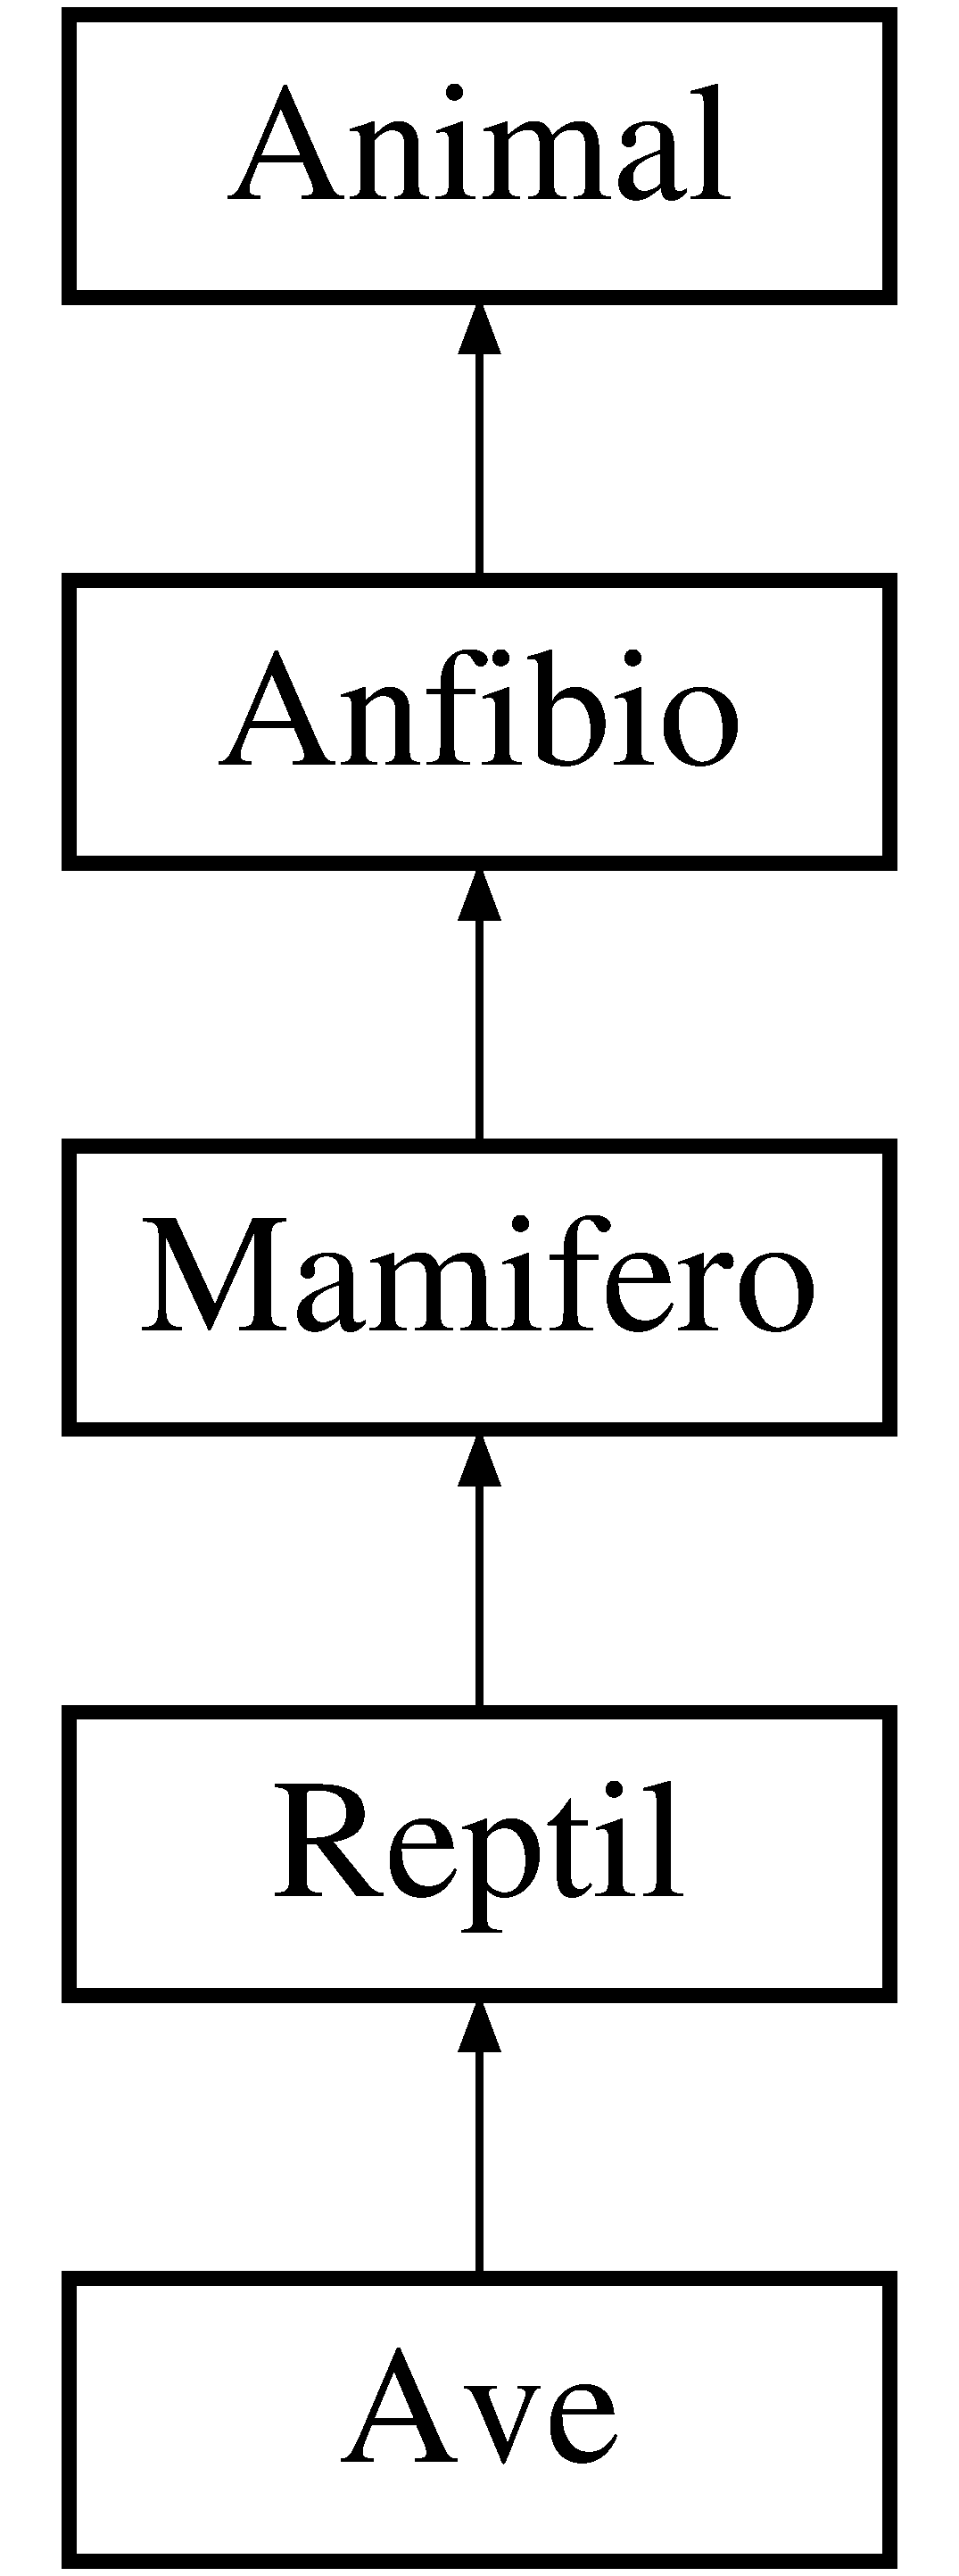
\includegraphics[height=5.000000cm]{class_anfibio}
\end{center}
\end{figure}
\subsection*{Public Member Functions}
\begin{DoxyCompactItemize}
\item 
\mbox{\hyperlink{class_anfibio_a91fd9b91b9124ab41ea9e9c9bb013476}{Anfibio}} ()
\begin{DoxyCompactList}\small\item\em Criação do Contrutor e Destrutor. \end{DoxyCompactList}\item 
void \mbox{\hyperlink{class_anfibio_a2efef746a06025c1b75c29c62f23909d}{Set\+Id}} (int id\+\_\+)
\begin{DoxyCompactList}\small\item\em Criação dos métodos Setters. \end{DoxyCompactList}\item 
\mbox{\Hypertarget{class_anfibio_af33d573093b0c426b92f94fce9fffed8}\label{class_anfibio_af33d573093b0c426b92f94fce9fffed8}} 
void \mbox{\hyperlink{class_anfibio_af33d573093b0c426b92f94fce9fffed8}{Set\+Classe}} (string classe\+\_\+)
\begin{DoxyCompactList}\small\item\em Chamada do metodo \mbox{\hyperlink{class_anfibio_af33d573093b0c426b92f94fce9fffed8}{Set\+Classe()}} \end{DoxyCompactList}\item 
\mbox{\Hypertarget{class_anfibio_a04a14e96798b0e7372c523851649b3bf}\label{class_anfibio_a04a14e96798b0e7372c523851649b3bf}} 
void \mbox{\hyperlink{class_anfibio_a04a14e96798b0e7372c523851649b3bf}{Set\+Nome}} (string nome\+\_\+)
\begin{DoxyCompactList}\small\item\em Chamada do metodo \mbox{\hyperlink{class_anfibio_a04a14e96798b0e7372c523851649b3bf}{Set\+Nome()}} \end{DoxyCompactList}\item 
\mbox{\Hypertarget{class_anfibio_a00eeb256834dbcd4601b2e82a5a22d5c}\label{class_anfibio_a00eeb256834dbcd4601b2e82a5a22d5c}} 
void \mbox{\hyperlink{class_anfibio_a00eeb256834dbcd4601b2e82a5a22d5c}{Set\+Cientifico}} (string cientifico\+\_\+)
\begin{DoxyCompactList}\small\item\em Chamada do metodo \mbox{\hyperlink{class_anfibio_a00eeb256834dbcd4601b2e82a5a22d5c}{Set\+Cientifico()}} \end{DoxyCompactList}\item 
\mbox{\Hypertarget{class_anfibio_acc02cae7ba5656abf06ecf9ac851b8f8}\label{class_anfibio_acc02cae7ba5656abf06ecf9ac851b8f8}} 
void \mbox{\hyperlink{class_anfibio_acc02cae7ba5656abf06ecf9ac851b8f8}{Set\+Sexo}} (string sexo\+\_\+)
\begin{DoxyCompactList}\small\item\em Chamada do metodo \mbox{\hyperlink{class_anfibio_acc02cae7ba5656abf06ecf9ac851b8f8}{Set\+Sexo()}} \end{DoxyCompactList}\item 
\mbox{\Hypertarget{class_anfibio_a965a795da7d5909264c62d5864d90e9f}\label{class_anfibio_a965a795da7d5909264c62d5864d90e9f}} 
void \mbox{\hyperlink{class_anfibio_a965a795da7d5909264c62d5864d90e9f}{Set\+Tamanho}} (float tamanho\+\_\+)
\begin{DoxyCompactList}\small\item\em Chamada do metodo \mbox{\hyperlink{class_anfibio_a965a795da7d5909264c62d5864d90e9f}{Set\+Tamanho()}} \end{DoxyCompactList}\item 
\mbox{\Hypertarget{class_anfibio_a8ccb409ba5e4faaab7e03425d77bc0fb}\label{class_anfibio_a8ccb409ba5e4faaab7e03425d77bc0fb}} 
void \mbox{\hyperlink{class_anfibio_a8ccb409ba5e4faaab7e03425d77bc0fb}{Set\+Dieta}} (string dieta\+\_\+)
\begin{DoxyCompactList}\small\item\em Chamada do metodo \mbox{\hyperlink{class_anfibio_a8ccb409ba5e4faaab7e03425d77bc0fb}{Set\+Dieta()}} \end{DoxyCompactList}\item 
\mbox{\Hypertarget{class_anfibio_a28e9be44ac5c33893861e17c37f47dab}\label{class_anfibio_a28e9be44ac5c33893861e17c37f47dab}} 
void \mbox{\hyperlink{class_anfibio_a28e9be44ac5c33893861e17c37f47dab}{Set\+Veterinario}} (int veterinario\+\_\+)
\begin{DoxyCompactList}\small\item\em Chamada do metodo \mbox{\hyperlink{class_anfibio_a28e9be44ac5c33893861e17c37f47dab}{Set\+Veterinario()}} \end{DoxyCompactList}\item 
\mbox{\Hypertarget{class_anfibio_a457f9740bfcc64ce5cdf4a861e452455}\label{class_anfibio_a457f9740bfcc64ce5cdf4a861e452455}} 
void \mbox{\hyperlink{class_anfibio_a457f9740bfcc64ce5cdf4a861e452455}{Set\+Tratador}} (int tratador\+\_\+)
\begin{DoxyCompactList}\small\item\em Chamada do metodo \mbox{\hyperlink{class_anfibio_a457f9740bfcc64ce5cdf4a861e452455}{Set\+Tratador()}} \end{DoxyCompactList}\item 
\mbox{\Hypertarget{class_anfibio_acd9cc4d047b66b880324fb5f9da5e32c}\label{class_anfibio_acd9cc4d047b66b880324fb5f9da5e32c}} 
void \mbox{\hyperlink{class_anfibio_acd9cc4d047b66b880324fb5f9da5e32c}{Set\+Batismo}} (string batismo\+\_\+)
\begin{DoxyCompactList}\small\item\em Chamada do metodo \mbox{\hyperlink{class_anfibio_acd9cc4d047b66b880324fb5f9da5e32c}{Set\+Batismo()}} \end{DoxyCompactList}\item 
\mbox{\Hypertarget{class_anfibio_a0cbd78686caf1e36795f2c56a776d867}\label{class_anfibio_a0cbd78686caf1e36795f2c56a776d867}} 
void \mbox{\hyperlink{class_anfibio_a0cbd78686caf1e36795f2c56a776d867}{Set\+Total}} (int total\+\_\+)
\begin{DoxyCompactList}\small\item\em Chamada do metodo \mbox{\hyperlink{class_anfibio_a0cbd78686caf1e36795f2c56a776d867}{Set\+Total()}} \end{DoxyCompactList}\item 
\mbox{\Hypertarget{class_anfibio_aef72a726adc5c20c02b8269a290dcd94}\label{class_anfibio_aef72a726adc5c20c02b8269a290dcd94}} 
void \mbox{\hyperlink{class_anfibio_aef72a726adc5c20c02b8269a290dcd94}{Set\+Ultima}} (int ultima\+\_\+)
\begin{DoxyCompactList}\small\item\em Chamada do metodo \mbox{\hyperlink{class_anfibio_aef72a726adc5c20c02b8269a290dcd94}{Set\+Ultima()}} \end{DoxyCompactList}\item 
int \mbox{\hyperlink{class_anfibio_a88b335b835421e611f5e0705208781a0}{Get\+Id}} (void)
\begin{DoxyCompactList}\small\item\em Criação dos métodos Getters. \end{DoxyCompactList}\item 
\mbox{\Hypertarget{class_anfibio_a0e33964b0b8e576cbf0b1f889e254cad}\label{class_anfibio_a0e33964b0b8e576cbf0b1f889e254cad}} 
string \mbox{\hyperlink{class_anfibio_a0e33964b0b8e576cbf0b1f889e254cad}{Get\+Classe}} (void)
\begin{DoxyCompactList}\small\item\em Chamada do metodo \mbox{\hyperlink{class_anfibio_a0e33964b0b8e576cbf0b1f889e254cad}{Get\+Classe()}} \end{DoxyCompactList}\item 
\mbox{\Hypertarget{class_anfibio_a36fe4e45be7a9477948d44d40c814205}\label{class_anfibio_a36fe4e45be7a9477948d44d40c814205}} 
string \mbox{\hyperlink{class_anfibio_a36fe4e45be7a9477948d44d40c814205}{Get\+Nome}} (void)
\begin{DoxyCompactList}\small\item\em Chamada do metodo \mbox{\hyperlink{class_anfibio_a36fe4e45be7a9477948d44d40c814205}{Get\+Nome()}} \end{DoxyCompactList}\item 
\mbox{\Hypertarget{class_anfibio_a8e8c536d4cc6e6f6b99cd1d7f3320344}\label{class_anfibio_a8e8c536d4cc6e6f6b99cd1d7f3320344}} 
string \mbox{\hyperlink{class_anfibio_a8e8c536d4cc6e6f6b99cd1d7f3320344}{Get\+Cientifico}} (void)
\begin{DoxyCompactList}\small\item\em Chamada do metodo \mbox{\hyperlink{class_anfibio_a8e8c536d4cc6e6f6b99cd1d7f3320344}{Get\+Cientifico()}} \end{DoxyCompactList}\item 
\mbox{\Hypertarget{class_anfibio_a61ad36eb6d5ce4ab2036f116eac167aa}\label{class_anfibio_a61ad36eb6d5ce4ab2036f116eac167aa}} 
string \mbox{\hyperlink{class_anfibio_a61ad36eb6d5ce4ab2036f116eac167aa}{Get\+Sexo}} (void)
\begin{DoxyCompactList}\small\item\em Chamada do metodo \mbox{\hyperlink{class_anfibio_a61ad36eb6d5ce4ab2036f116eac167aa}{Get\+Sexo()}} \end{DoxyCompactList}\item 
\mbox{\Hypertarget{class_anfibio_a68248d0111d0699c570762dd14b7163a}\label{class_anfibio_a68248d0111d0699c570762dd14b7163a}} 
float \mbox{\hyperlink{class_anfibio_a68248d0111d0699c570762dd14b7163a}{Get\+Tamanho}} (void)
\begin{DoxyCompactList}\small\item\em Chamada do metodo \mbox{\hyperlink{class_anfibio_a68248d0111d0699c570762dd14b7163a}{Get\+Tamanho()}} \end{DoxyCompactList}\item 
\mbox{\Hypertarget{class_anfibio_adabeacbe469bd305ecb8fb21328523b6}\label{class_anfibio_adabeacbe469bd305ecb8fb21328523b6}} 
string \mbox{\hyperlink{class_anfibio_adabeacbe469bd305ecb8fb21328523b6}{Get\+Dieta}} (void)
\begin{DoxyCompactList}\small\item\em Chamada do metodo \mbox{\hyperlink{class_anfibio_adabeacbe469bd305ecb8fb21328523b6}{Get\+Dieta()}} \end{DoxyCompactList}\item 
\mbox{\Hypertarget{class_anfibio_a923b28f7a27724fd9fba0856d4fc7f76}\label{class_anfibio_a923b28f7a27724fd9fba0856d4fc7f76}} 
int \mbox{\hyperlink{class_anfibio_a923b28f7a27724fd9fba0856d4fc7f76}{Get\+Veterinario}} (void)
\begin{DoxyCompactList}\small\item\em Chamada do metodo \mbox{\hyperlink{class_anfibio_a923b28f7a27724fd9fba0856d4fc7f76}{Get\+Veterinario()}} \end{DoxyCompactList}\item 
\mbox{\Hypertarget{class_anfibio_af0be74ef5f7cf1b51564350d17d2683d}\label{class_anfibio_af0be74ef5f7cf1b51564350d17d2683d}} 
int \mbox{\hyperlink{class_anfibio_af0be74ef5f7cf1b51564350d17d2683d}{Get\+Tratador}} (void)
\begin{DoxyCompactList}\small\item\em Chamada do metodo \mbox{\hyperlink{class_anfibio_af0be74ef5f7cf1b51564350d17d2683d}{Get\+Tratador()}} \end{DoxyCompactList}\item 
\mbox{\Hypertarget{class_anfibio_ad68274710837e3453769181b8cc2c1de}\label{class_anfibio_ad68274710837e3453769181b8cc2c1de}} 
string \mbox{\hyperlink{class_anfibio_ad68274710837e3453769181b8cc2c1de}{Get\+Batismo}} (void)
\begin{DoxyCompactList}\small\item\em Chamada do metodo \mbox{\hyperlink{class_anfibio_ad68274710837e3453769181b8cc2c1de}{Get\+Batismo()}} \end{DoxyCompactList}\item 
\mbox{\Hypertarget{class_anfibio_a6d2f6c8090371f63615cb74868396c06}\label{class_anfibio_a6d2f6c8090371f63615cb74868396c06}} 
int \mbox{\hyperlink{class_anfibio_a6d2f6c8090371f63615cb74868396c06}{Get\+Total}} (void)
\begin{DoxyCompactList}\small\item\em Chamada do metodo \mbox{\hyperlink{class_anfibio_a6d2f6c8090371f63615cb74868396c06}{Get\+Total()}} \end{DoxyCompactList}\item 
\mbox{\Hypertarget{class_anfibio_a41391515ad316e2bc3215328f25ed8ea}\label{class_anfibio_a41391515ad316e2bc3215328f25ed8ea}} 
string \mbox{\hyperlink{class_anfibio_a41391515ad316e2bc3215328f25ed8ea}{Get\+Ultima}} (void)
\begin{DoxyCompactList}\small\item\em Chamada do metodo \mbox{\hyperlink{class_anfibio_a41391515ad316e2bc3215328f25ed8ea}{Get\+Ultima()}} \end{DoxyCompactList}\end{DoxyCompactItemize}
\subsection*{Protected Attributes}
\begin{DoxyCompactItemize}
\item 
int \mbox{\hyperlink{class_anfibio_a46768866ac5b9ab108219631ea4cbfc6}{total\+\_\+mudas}}
\begin{DoxyCompactList}\small\item\em Criação dos parâmetros da classe \mbox{\hyperlink{class_anfibio}{Anfibio}}. \end{DoxyCompactList}\item 
\mbox{\Hypertarget{class_anfibio_a1aad121d75a27621d2dc8be39cf14123}\label{class_anfibio_a1aad121d75a27621d2dc8be39cf14123}} 
string {\bfseries ultima\+\_\+muda}
\end{DoxyCompactItemize}
\subsection*{Additional Inherited Members}


\subsection{Detailed Description}
Criação da classe \mbox{\hyperlink{class_anfibio}{Anfibio}}. 

A classe \mbox{\hyperlink{class_anfibio}{Anfibio}} herda os parâmetros da classe \mbox{\hyperlink{class_animal}{Animal}} 

\subsection{Constructor \& Destructor Documentation}
\mbox{\Hypertarget{class_anfibio_a91fd9b91b9124ab41ea9e9c9bb013476}\label{class_anfibio_a91fd9b91b9124ab41ea9e9c9bb013476}} 
\index{Anfibio@{Anfibio}!Anfibio@{Anfibio}}
\index{Anfibio@{Anfibio}!Anfibio@{Anfibio}}
\subsubsection{\texorpdfstring{Anfibio()}{Anfibio()}}
{\footnotesize\ttfamily Anfibio\+::\+Anfibio (\begin{DoxyParamCaption}{ }\end{DoxyParamCaption})}



Criação do Contrutor e Destrutor. 

Chamada do contrutor e destrutor() 

\subsection{Member Function Documentation}
\mbox{\Hypertarget{class_anfibio_a88b335b835421e611f5e0705208781a0}\label{class_anfibio_a88b335b835421e611f5e0705208781a0}} 
\index{Anfibio@{Anfibio}!Get\+Id@{Get\+Id}}
\index{Get\+Id@{Get\+Id}!Anfibio@{Anfibio}}
\subsubsection{\texorpdfstring{Get\+Id()}{GetId()}}
{\footnotesize\ttfamily int Anfibio\+::\+Get\+Id (\begin{DoxyParamCaption}\item[{void}]{ }\end{DoxyParamCaption})}



Criação dos métodos Getters. 

Chamada do metodo \mbox{\hyperlink{class_anfibio_a88b335b835421e611f5e0705208781a0}{Get\+Id()}} \mbox{\Hypertarget{class_anfibio_a2efef746a06025c1b75c29c62f23909d}\label{class_anfibio_a2efef746a06025c1b75c29c62f23909d}} 
\index{Anfibio@{Anfibio}!Set\+Id@{Set\+Id}}
\index{Set\+Id@{Set\+Id}!Anfibio@{Anfibio}}
\subsubsection{\texorpdfstring{Set\+Id()}{SetId()}}
{\footnotesize\ttfamily void Anfibio\+::\+Set\+Id (\begin{DoxyParamCaption}\item[{int}]{id\+\_\+ }\end{DoxyParamCaption})}



Criação dos métodos Setters. 

Chamada do metodo \mbox{\hyperlink{class_anfibio_a2efef746a06025c1b75c29c62f23909d}{Set\+Id()}} 

\subsection{Member Data Documentation}
\mbox{\Hypertarget{class_anfibio_a46768866ac5b9ab108219631ea4cbfc6}\label{class_anfibio_a46768866ac5b9ab108219631ea4cbfc6}} 
\index{Anfibio@{Anfibio}!total\+\_\+mudas@{total\+\_\+mudas}}
\index{total\+\_\+mudas@{total\+\_\+mudas}!Anfibio@{Anfibio}}
\subsubsection{\texorpdfstring{total\+\_\+mudas}{total\_mudas}}
{\footnotesize\ttfamily int Anfibio\+::total\+\_\+mudas\hspace{0.3cm}{\ttfamily [protected]}}



Criação dos parâmetros da classe \mbox{\hyperlink{class_anfibio}{Anfibio}}. 


\begin{DoxyParams}{Parameters}
{\em int} & total\+\_\+mudas para guardar o o total de mudas \\
\hline
{\em string} & ultima\+\_\+muda para guardar a ultima muda \\
\hline
\end{DoxyParams}


The documentation for this class was generated from the following files\+:\begin{DoxyCompactItemize}
\item 
doxygen/anfibio.\+h\item 
doxygen/anfibio.\+cpp\end{DoxyCompactItemize}

\hypertarget{class_animal}{}\section{Animal Class Reference}
\label{class_animal}\index{Animal@{Animal}}


Criação da classe \mbox{\hyperlink{class_animal}{Animal}}.  




{\ttfamily \#include $<$animal.\+h$>$}

Inheritance diagram for Animal\+:\begin{figure}[H]
\begin{center}
\leavevmode
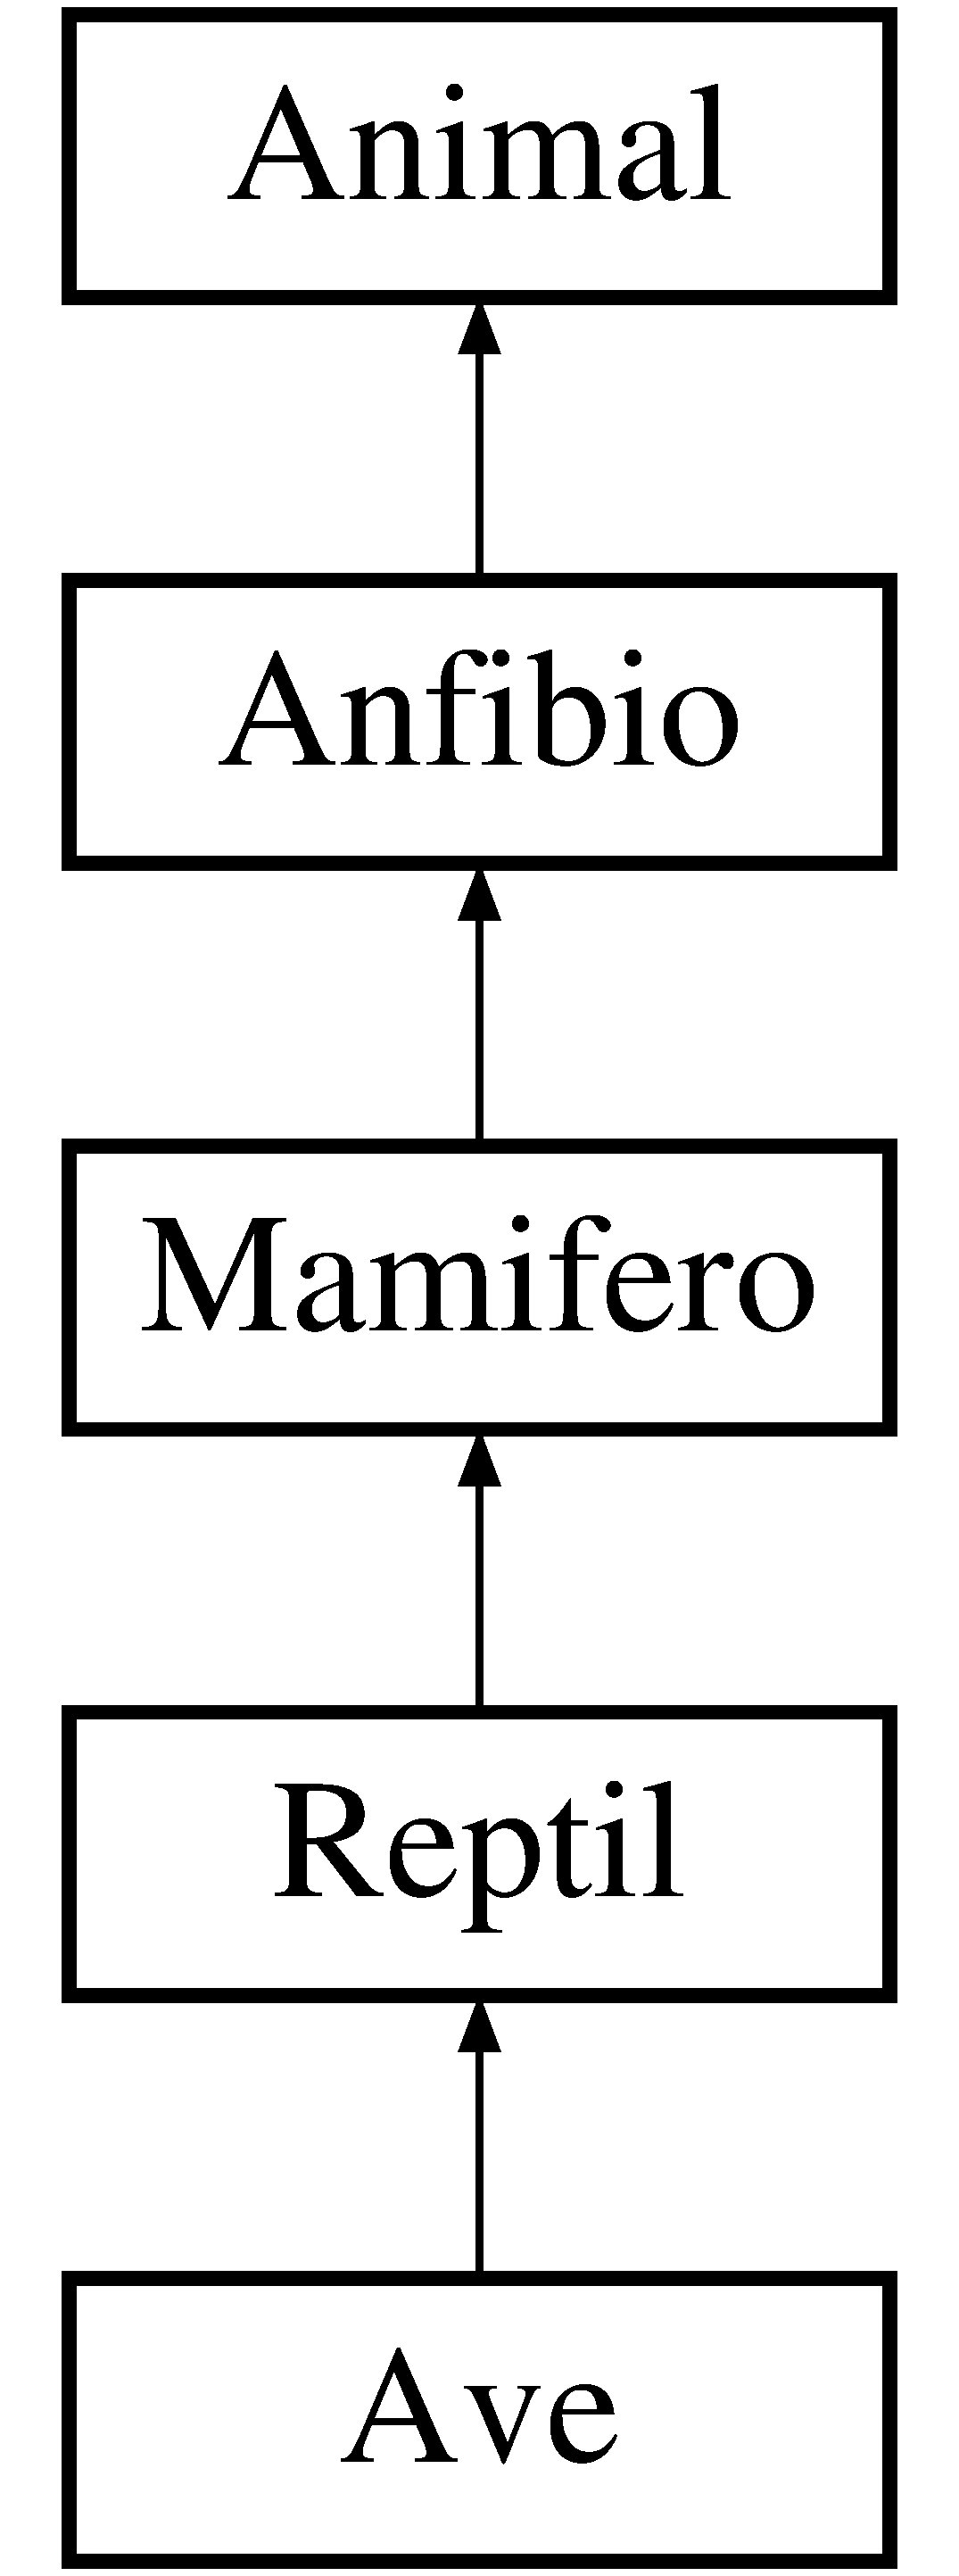
\includegraphics[height=5.000000cm]{class_animal}
\end{center}
\end{figure}
\subsection*{Protected Member Functions}
\begin{DoxyCompactItemize}
\item 
\mbox{\hyperlink{class_animal_a1e726a49ec952443190ac62dad22353c}{Animal}} ()
\begin{DoxyCompactList}\small\item\em Criação dos parâmetros da classe \mbox{\hyperlink{class_animal}{Animal}}. \end{DoxyCompactList}\end{DoxyCompactItemize}
\subsection*{Protected Attributes}
\begin{DoxyCompactItemize}
\item 
\mbox{\Hypertarget{class_animal_a0e1e797aa638af5d8276bcf12fad9a1f}\label{class_animal_a0e1e797aa638af5d8276bcf12fad9a1f}} 
int {\bfseries id}
\item 
\mbox{\Hypertarget{class_animal_ac18558124618675ac262369adcd6e2f5}\label{class_animal_ac18558124618675ac262369adcd6e2f5}} 
string {\bfseries classe}
\item 
\mbox{\Hypertarget{class_animal_a54f3f22208c7342039266c8c87de99e7}\label{class_animal_a54f3f22208c7342039266c8c87de99e7}} 
string {\bfseries nome}
\item 
\mbox{\Hypertarget{class_animal_afb1c2c6e57afabb641cfac58307a54d7}\label{class_animal_afb1c2c6e57afabb641cfac58307a54d7}} 
string {\bfseries cientifico}
\item 
\mbox{\Hypertarget{class_animal_ae606d25f0901c7780603b5b15d0dc763}\label{class_animal_ae606d25f0901c7780603b5b15d0dc763}} 
string {\bfseries sexo}
\item 
\mbox{\Hypertarget{class_animal_af164439fb6b2f4c470f451a8e7cbfd1e}\label{class_animal_af164439fb6b2f4c470f451a8e7cbfd1e}} 
float {\bfseries tamanho}
\item 
\mbox{\Hypertarget{class_animal_a1d9c10e256acf2b2dfdf5b57c135af54}\label{class_animal_a1d9c10e256acf2b2dfdf5b57c135af54}} 
string {\bfseries dieta}
\item 
\mbox{\Hypertarget{class_animal_af012f0c22d494aa3ebfb19e2d571b8b7}\label{class_animal_af012f0c22d494aa3ebfb19e2d571b8b7}} 
int {\bfseries veterinario}
\item 
\mbox{\Hypertarget{class_animal_adf6d91811fe24cbc75f253cce86393e0}\label{class_animal_adf6d91811fe24cbc75f253cce86393e0}} 
int {\bfseries tratador}
\item 
\mbox{\Hypertarget{class_animal_aca7799bebd7ead41bca479831a57a2be}\label{class_animal_aca7799bebd7ead41bca479831a57a2be}} 
string {\bfseries batismo}
\end{DoxyCompactItemize}


\subsection{Detailed Description}
Criação da classe \mbox{\hyperlink{class_animal}{Animal}}. 

\subsection{Constructor \& Destructor Documentation}
\mbox{\Hypertarget{class_animal_a1e726a49ec952443190ac62dad22353c}\label{class_animal_a1e726a49ec952443190ac62dad22353c}} 
\index{Animal@{Animal}!Animal@{Animal}}
\index{Animal@{Animal}!Animal@{Animal}}
\subsubsection{\texorpdfstring{Animal()}{Animal()}}
{\footnotesize\ttfamily Animal\+::\+Animal (\begin{DoxyParamCaption}{ }\end{DoxyParamCaption})\hspace{0.3cm}{\ttfamily [inline]}, {\ttfamily [protected]}}



Criação dos parâmetros da classe \mbox{\hyperlink{class_animal}{Animal}}. 


\begin{DoxyParams}{Parameters}
{\em int} & id para guardar o id do animal \\
\hline
{\em string} & classe para a classe do animal \\
\hline
{\em string} & nome guarda o nome do animal \\
\hline
{\em string} & cientifico guarda o termo cientifico do animal \\
\hline
{\em char} & sexo guarda o sexo do animal \\
\hline
{\em float} & tamanho guarda o tamanho do animal \\
\hline
{\em string} & dieta guarda a dieta do animal \\
\hline
{\em int} & veterinario verifica se tem algum veterinario tratando o animal \\
\hline
{\em int} & tratador verifica se tem algum tratador tratando o animal \\
\hline
{\em string} & batismo guarda o nome de batismo do animal \\
\hline
\end{DoxyParams}


The documentation for this class was generated from the following file\+:\begin{DoxyCompactItemize}
\item 
doxygen/animal.\+h\end{DoxyCompactItemize}

\hypertarget{class_ave}{}\section{Ave Class Reference}
\label{class_ave}\index{Ave@{Ave}}


Criação da classe \mbox{\hyperlink{class_ave}{Ave}}.  




{\ttfamily \#include $<$ave.\+h$>$}

Inheritance diagram for Ave\+:\begin{figure}[H]
\begin{center}
\leavevmode
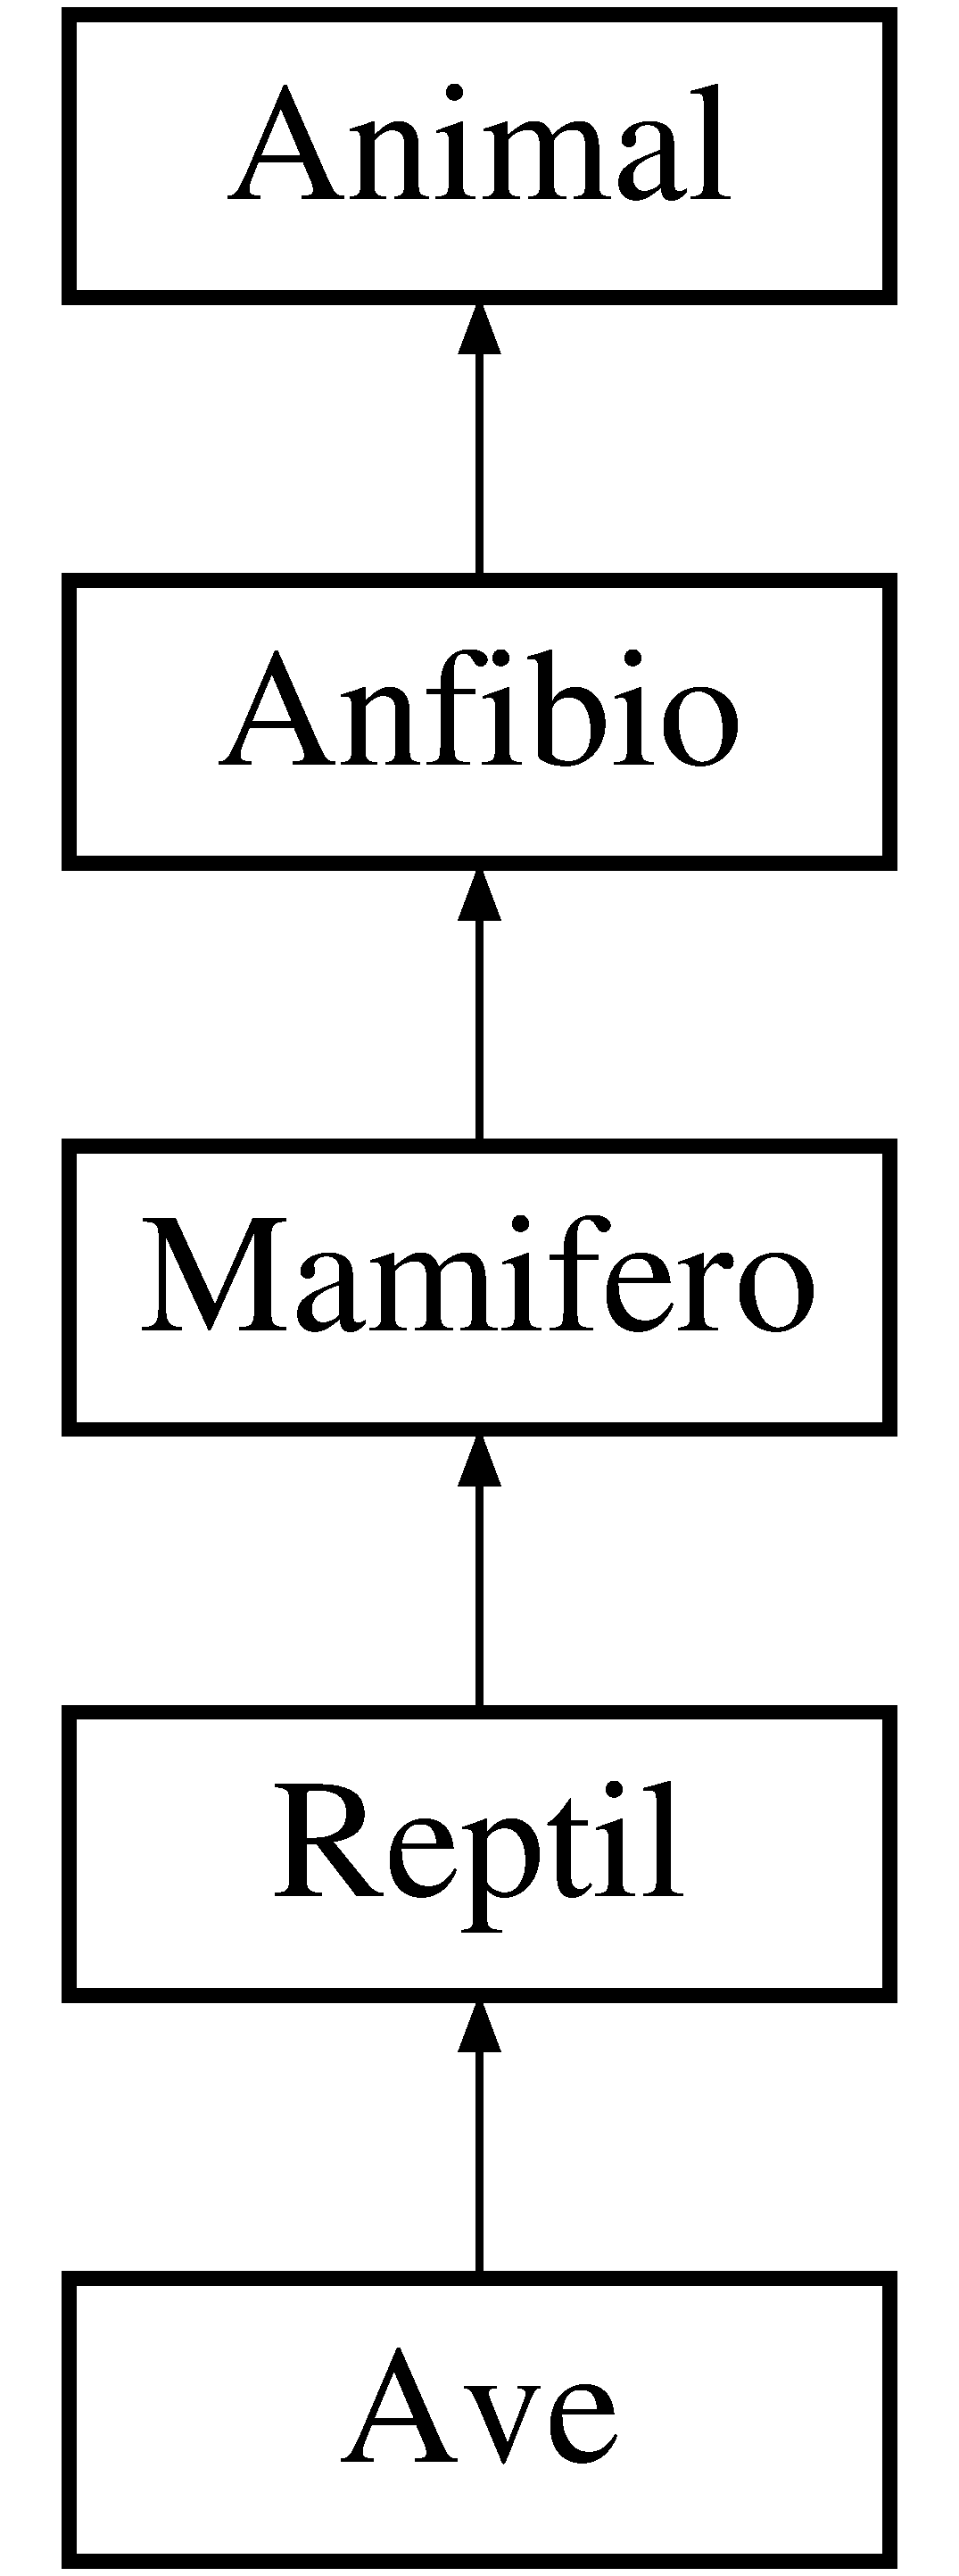
\includegraphics[height=5.000000cm]{class_ave}
\end{center}
\end{figure}
\subsection*{Public Member Functions}
\begin{DoxyCompactItemize}
\item 
\mbox{\hyperlink{class_ave_a31bc97c3258df566381300c8b9abc73a}{Ave}} ()
\begin{DoxyCompactList}\small\item\em Criação do Contrutor e Destrutor. \end{DoxyCompactList}\item 
void \mbox{\hyperlink{class_ave_add888c033de541a44c5c31a31db5ad1d}{Set\+Id}} (int id\+\_\+)
\begin{DoxyCompactList}\small\item\em Criação dos métodos Setters. \end{DoxyCompactList}\item 
\mbox{\Hypertarget{class_ave_ae393103817453e9165a9ff7fb6a73bd9}\label{class_ave_ae393103817453e9165a9ff7fb6a73bd9}} 
void \mbox{\hyperlink{class_ave_ae393103817453e9165a9ff7fb6a73bd9}{Set\+Classe}} (string classe\+\_\+)
\begin{DoxyCompactList}\small\item\em Chamada do metodo \mbox{\hyperlink{class_ave_ae393103817453e9165a9ff7fb6a73bd9}{Set\+Classe()}} \end{DoxyCompactList}\item 
\mbox{\Hypertarget{class_ave_a577d65a227548e30ced15c41706d38ae}\label{class_ave_a577d65a227548e30ced15c41706d38ae}} 
void \mbox{\hyperlink{class_ave_a577d65a227548e30ced15c41706d38ae}{Set\+Nome}} (string nome\+\_\+)
\begin{DoxyCompactList}\small\item\em Chamada do metodo \mbox{\hyperlink{class_ave_a577d65a227548e30ced15c41706d38ae}{Set\+Nome()}} \end{DoxyCompactList}\item 
\mbox{\Hypertarget{class_ave_a4e3b9ce1813889f3c89ad68100a2e297}\label{class_ave_a4e3b9ce1813889f3c89ad68100a2e297}} 
void \mbox{\hyperlink{class_ave_a4e3b9ce1813889f3c89ad68100a2e297}{Set\+Cientifico}} (string cientifico\+\_\+)
\begin{DoxyCompactList}\small\item\em Chamada do metodo \mbox{\hyperlink{class_ave_a4e3b9ce1813889f3c89ad68100a2e297}{Set\+Cientifico()}} \end{DoxyCompactList}\item 
\mbox{\Hypertarget{class_ave_a96c89cec0539097e96fbfd77a87d59c2}\label{class_ave_a96c89cec0539097e96fbfd77a87d59c2}} 
void \mbox{\hyperlink{class_ave_a96c89cec0539097e96fbfd77a87d59c2}{Set\+Sexo}} (string sexo\+\_\+)
\begin{DoxyCompactList}\small\item\em Chamada do metodo \mbox{\hyperlink{class_ave_a96c89cec0539097e96fbfd77a87d59c2}{Set\+Sexo()}} \end{DoxyCompactList}\item 
\mbox{\Hypertarget{class_ave_a5b83fc1a6189ea2fbe72789fd27f2637}\label{class_ave_a5b83fc1a6189ea2fbe72789fd27f2637}} 
void \mbox{\hyperlink{class_ave_a5b83fc1a6189ea2fbe72789fd27f2637}{Set\+Tamanho}} (float tamanho\+\_\+)
\begin{DoxyCompactList}\small\item\em Chamada do metodo \mbox{\hyperlink{class_ave_a5b83fc1a6189ea2fbe72789fd27f2637}{Set\+Tamanho()}} \end{DoxyCompactList}\item 
\mbox{\Hypertarget{class_ave_abae4d4e57ba2ef8f043d937b1fe0074e}\label{class_ave_abae4d4e57ba2ef8f043d937b1fe0074e}} 
void \mbox{\hyperlink{class_ave_abae4d4e57ba2ef8f043d937b1fe0074e}{Set\+Dieta}} (string dieta\+\_\+)
\begin{DoxyCompactList}\small\item\em Chamada do metodo \mbox{\hyperlink{class_ave_abae4d4e57ba2ef8f043d937b1fe0074e}{Set\+Dieta()}} \end{DoxyCompactList}\item 
\mbox{\Hypertarget{class_ave_ad382a03d23a444e7288e2825f1af08db}\label{class_ave_ad382a03d23a444e7288e2825f1af08db}} 
void \mbox{\hyperlink{class_ave_ad382a03d23a444e7288e2825f1af08db}{Set\+Veterinario}} (int veterinario\+\_\+)
\begin{DoxyCompactList}\small\item\em Chamada do metodo \mbox{\hyperlink{class_ave_ad382a03d23a444e7288e2825f1af08db}{Set\+Veterinario()}} \end{DoxyCompactList}\item 
\mbox{\Hypertarget{class_ave_ae82166abb8f2492f431519fdcf25cb40}\label{class_ave_ae82166abb8f2492f431519fdcf25cb40}} 
void \mbox{\hyperlink{class_ave_ae82166abb8f2492f431519fdcf25cb40}{Set\+Tratador}} (int tratador\+\_\+)
\begin{DoxyCompactList}\small\item\em Chamada do metodo \mbox{\hyperlink{class_ave_ae82166abb8f2492f431519fdcf25cb40}{Set\+Tratador()}} \end{DoxyCompactList}\item 
\mbox{\Hypertarget{class_ave_a9e414f7bb59aae864f313b4be840d49c}\label{class_ave_a9e414f7bb59aae864f313b4be840d49c}} 
void \mbox{\hyperlink{class_ave_a9e414f7bb59aae864f313b4be840d49c}{Set\+Batismo}} (string batismo)
\begin{DoxyCompactList}\small\item\em Chamada do metodo \mbox{\hyperlink{class_ave_a9e414f7bb59aae864f313b4be840d49c}{Set\+Batismo()}} \end{DoxyCompactList}\item 
\mbox{\Hypertarget{class_ave_a65e15e29bf02bb6842ca16e6d5b18708}\label{class_ave_a65e15e29bf02bb6842ca16e6d5b18708}} 
void \mbox{\hyperlink{class_ave_a65e15e29bf02bb6842ca16e6d5b18708}{Set\+Tamanho\+Bico}} (float tamanho\+\_\+bico\+\_\+)
\begin{DoxyCompactList}\small\item\em Chamada do metodo \mbox{\hyperlink{class_ave_a65e15e29bf02bb6842ca16e6d5b18708}{Set\+Tamanho\+Bico()}} \end{DoxyCompactList}\item 
\mbox{\Hypertarget{class_ave_aa5180cce1170f89f2d8cb547a4871dd8}\label{class_ave_aa5180cce1170f89f2d8cb547a4871dd8}} 
void \mbox{\hyperlink{class_ave_aa5180cce1170f89f2d8cb547a4871dd8}{Set\+Envergadura}} (float envergadura\+\_\+)
\begin{DoxyCompactList}\small\item\em Chamada do metodo \mbox{\hyperlink{class_ave_aa5180cce1170f89f2d8cb547a4871dd8}{Set\+Envergadura()}} \end{DoxyCompactList}\item 
int \mbox{\hyperlink{class_ave_a5c3d1e3b7b356a08b2fddd242c2fa426}{Get\+Id}} (void)
\begin{DoxyCompactList}\small\item\em Criação dos métodos Getters. \end{DoxyCompactList}\item 
\mbox{\Hypertarget{class_ave_a1bea1200baf9ecc47899b6797a86c675}\label{class_ave_a1bea1200baf9ecc47899b6797a86c675}} 
string \mbox{\hyperlink{class_ave_a1bea1200baf9ecc47899b6797a86c675}{Get\+Classe}} (void)
\begin{DoxyCompactList}\small\item\em Chamada do metodo \mbox{\hyperlink{class_ave_a1bea1200baf9ecc47899b6797a86c675}{Get\+Classe()}} \end{DoxyCompactList}\item 
\mbox{\Hypertarget{class_ave_ae9085c0c2d1ac90fa5c659f15ac7955d}\label{class_ave_ae9085c0c2d1ac90fa5c659f15ac7955d}} 
string \mbox{\hyperlink{class_ave_ae9085c0c2d1ac90fa5c659f15ac7955d}{Get\+Nome}} (void)
\begin{DoxyCompactList}\small\item\em Chamada do metodo \mbox{\hyperlink{class_ave_ae9085c0c2d1ac90fa5c659f15ac7955d}{Get\+Nome()}} \end{DoxyCompactList}\item 
\mbox{\Hypertarget{class_ave_ac8f51606a52091a940e2fe8b81eee1c3}\label{class_ave_ac8f51606a52091a940e2fe8b81eee1c3}} 
string \mbox{\hyperlink{class_ave_ac8f51606a52091a940e2fe8b81eee1c3}{Get\+Cientifico}} (void)
\begin{DoxyCompactList}\small\item\em Chamada do metodo \mbox{\hyperlink{class_ave_ac8f51606a52091a940e2fe8b81eee1c3}{Get\+Cientifico()}} \end{DoxyCompactList}\item 
\mbox{\Hypertarget{class_ave_a8c629be919df2c2d5160456e7e68251d}\label{class_ave_a8c629be919df2c2d5160456e7e68251d}} 
string \mbox{\hyperlink{class_ave_a8c629be919df2c2d5160456e7e68251d}{Get\+Sexo}} (void)
\begin{DoxyCompactList}\small\item\em Chamada do metodo \mbox{\hyperlink{class_ave_a8c629be919df2c2d5160456e7e68251d}{Get\+Sexo()}} \end{DoxyCompactList}\item 
\mbox{\Hypertarget{class_ave_a6e5ae71a63a769725619ffa4f1c6bd15}\label{class_ave_a6e5ae71a63a769725619ffa4f1c6bd15}} 
float \mbox{\hyperlink{class_ave_a6e5ae71a63a769725619ffa4f1c6bd15}{Get\+Tamanho}} (void)
\begin{DoxyCompactList}\small\item\em Chamada do metodo \mbox{\hyperlink{class_ave_a6e5ae71a63a769725619ffa4f1c6bd15}{Get\+Tamanho()}} \end{DoxyCompactList}\item 
\mbox{\Hypertarget{class_ave_ab7b88331c601b8beb16969b0cc923b6f}\label{class_ave_ab7b88331c601b8beb16969b0cc923b6f}} 
string \mbox{\hyperlink{class_ave_ab7b88331c601b8beb16969b0cc923b6f}{Get\+Dieta}} (void)
\begin{DoxyCompactList}\small\item\em Chamada do metodo \mbox{\hyperlink{class_ave_ab7b88331c601b8beb16969b0cc923b6f}{Get\+Dieta()}} \end{DoxyCompactList}\item 
\mbox{\Hypertarget{class_ave_aad85251d6f3411c8d4f6ba0a099acf90}\label{class_ave_aad85251d6f3411c8d4f6ba0a099acf90}} 
int \mbox{\hyperlink{class_ave_aad85251d6f3411c8d4f6ba0a099acf90}{Get\+Veterinario}} (void)
\begin{DoxyCompactList}\small\item\em Chamada do metodo \mbox{\hyperlink{class_ave_aad85251d6f3411c8d4f6ba0a099acf90}{Get\+Veterinario()}} \end{DoxyCompactList}\item 
\mbox{\Hypertarget{class_ave_ac205b0f275e6647ad7ad4abbcb323912}\label{class_ave_ac205b0f275e6647ad7ad4abbcb323912}} 
int \mbox{\hyperlink{class_ave_ac205b0f275e6647ad7ad4abbcb323912}{Get\+Tratador}} (void)
\begin{DoxyCompactList}\small\item\em Chamada do metodo \mbox{\hyperlink{class_ave_ac205b0f275e6647ad7ad4abbcb323912}{Get\+Tratador()}} \end{DoxyCompactList}\item 
\mbox{\Hypertarget{class_ave_af6ff1f6baf664ffefa121372a3830f4f}\label{class_ave_af6ff1f6baf664ffefa121372a3830f4f}} 
string \mbox{\hyperlink{class_ave_af6ff1f6baf664ffefa121372a3830f4f}{Get\+Batismo}} (void)
\begin{DoxyCompactList}\small\item\em Chamada do metodo \mbox{\hyperlink{class_ave_af6ff1f6baf664ffefa121372a3830f4f}{Get\+Batismo()}} \end{DoxyCompactList}\item 
\mbox{\Hypertarget{class_ave_a2b2b43698ae468b9bb1c64174064313e}\label{class_ave_a2b2b43698ae468b9bb1c64174064313e}} 
float \mbox{\hyperlink{class_ave_a2b2b43698ae468b9bb1c64174064313e}{Get\+Tamanho\+Bico}} (void)
\begin{DoxyCompactList}\small\item\em Chamada do metodo \mbox{\hyperlink{class_ave_a2b2b43698ae468b9bb1c64174064313e}{Get\+Tamanho\+Bico()}} \end{DoxyCompactList}\item 
\mbox{\Hypertarget{class_ave_a91103e0a19d277bdd0b8fd41e86618ed}\label{class_ave_a91103e0a19d277bdd0b8fd41e86618ed}} 
float \mbox{\hyperlink{class_ave_a91103e0a19d277bdd0b8fd41e86618ed}{Get\+Envergadura}} (void)
\begin{DoxyCompactList}\small\item\em Chamada do metodo \mbox{\hyperlink{class_ave_a91103e0a19d277bdd0b8fd41e86618ed}{Get\+Envergadura()}} \end{DoxyCompactList}\end{DoxyCompactItemize}
\subsection*{Public Attributes}
\begin{DoxyCompactItemize}
\item 
float \mbox{\hyperlink{class_ave_a0285e182b8a55a290b10b621ed93602d}{tamanho\+\_\+bico}}
\begin{DoxyCompactList}\small\item\em Criação dos parâmetros da classe \mbox{\hyperlink{class_ave}{Ave}}. \end{DoxyCompactList}\item 
\mbox{\Hypertarget{class_ave_a6736c6a2391314daeb88e3e063c63ac0}\label{class_ave_a6736c6a2391314daeb88e3e063c63ac0}} 
float {\bfseries envergadura}
\end{DoxyCompactItemize}
\subsection*{Additional Inherited Members}


\subsection{Detailed Description}
Criação da classe \mbox{\hyperlink{class_ave}{Ave}}. 

A classe veterinário herda os parâmetros da classe \mbox{\hyperlink{class_reptil}{Reptil}} 

\subsection{Constructor \& Destructor Documentation}
\mbox{\Hypertarget{class_ave_a31bc97c3258df566381300c8b9abc73a}\label{class_ave_a31bc97c3258df566381300c8b9abc73a}} 
\index{Ave@{Ave}!Ave@{Ave}}
\index{Ave@{Ave}!Ave@{Ave}}
\subsubsection{\texorpdfstring{Ave()}{Ave()}}
{\footnotesize\ttfamily Ave\+::\+Ave (\begin{DoxyParamCaption}{ }\end{DoxyParamCaption})}



Criação do Contrutor e Destrutor. 

Chamada do contrutor e destrutor() 

\subsection{Member Function Documentation}
\mbox{\Hypertarget{class_ave_a5c3d1e3b7b356a08b2fddd242c2fa426}\label{class_ave_a5c3d1e3b7b356a08b2fddd242c2fa426}} 
\index{Ave@{Ave}!Get\+Id@{Get\+Id}}
\index{Get\+Id@{Get\+Id}!Ave@{Ave}}
\subsubsection{\texorpdfstring{Get\+Id()}{GetId()}}
{\footnotesize\ttfamily int Ave\+::\+Get\+Id (\begin{DoxyParamCaption}\item[{void}]{ }\end{DoxyParamCaption})}



Criação dos métodos Getters. 

Chamada do metodo \mbox{\hyperlink{class_ave_a5c3d1e3b7b356a08b2fddd242c2fa426}{Get\+Id()}} \mbox{\Hypertarget{class_ave_add888c033de541a44c5c31a31db5ad1d}\label{class_ave_add888c033de541a44c5c31a31db5ad1d}} 
\index{Ave@{Ave}!Set\+Id@{Set\+Id}}
\index{Set\+Id@{Set\+Id}!Ave@{Ave}}
\subsubsection{\texorpdfstring{Set\+Id()}{SetId()}}
{\footnotesize\ttfamily void Ave\+::\+Set\+Id (\begin{DoxyParamCaption}\item[{int}]{id\+\_\+ }\end{DoxyParamCaption})}



Criação dos métodos Setters. 

Chamada do metodo \mbox{\hyperlink{class_ave_add888c033de541a44c5c31a31db5ad1d}{Set\+Id()}} 

\subsection{Member Data Documentation}
\mbox{\Hypertarget{class_ave_a0285e182b8a55a290b10b621ed93602d}\label{class_ave_a0285e182b8a55a290b10b621ed93602d}} 
\index{Ave@{Ave}!tamanho\+\_\+bico@{tamanho\+\_\+bico}}
\index{tamanho\+\_\+bico@{tamanho\+\_\+bico}!Ave@{Ave}}
\subsubsection{\texorpdfstring{tamanho\+\_\+bico}{tamanho\_bico}}
{\footnotesize\ttfamily float Ave\+::tamanho\+\_\+bico}



Criação dos parâmetros da classe \mbox{\hyperlink{class_ave}{Ave}}. 


\begin{DoxyParams}{Parameters}
{\em float} & tamanho\+\_\+bico para guardar o tamanho do bico do animal \\
\hline
{\em float} & envergadura para guardar a envergadura do animal \\
\hline
\end{DoxyParams}


The documentation for this class was generated from the following files\+:\begin{DoxyCompactItemize}
\item 
doxygen/ave.\+h\item 
doxygen/ave.\+cpp\end{DoxyCompactItemize}

\hypertarget{class_erro_animal}{}\section{Erro\+Animal Class Reference}
\label{class_erro_animal}\index{Erro\+Animal@{Erro\+Animal}}


Um tratamento de excessão.  




{\ttfamily \#include $<$menu.\+h$>$}

Inheritance diagram for Erro\+Animal\+:\begin{figure}[H]
\begin{center}
\leavevmode
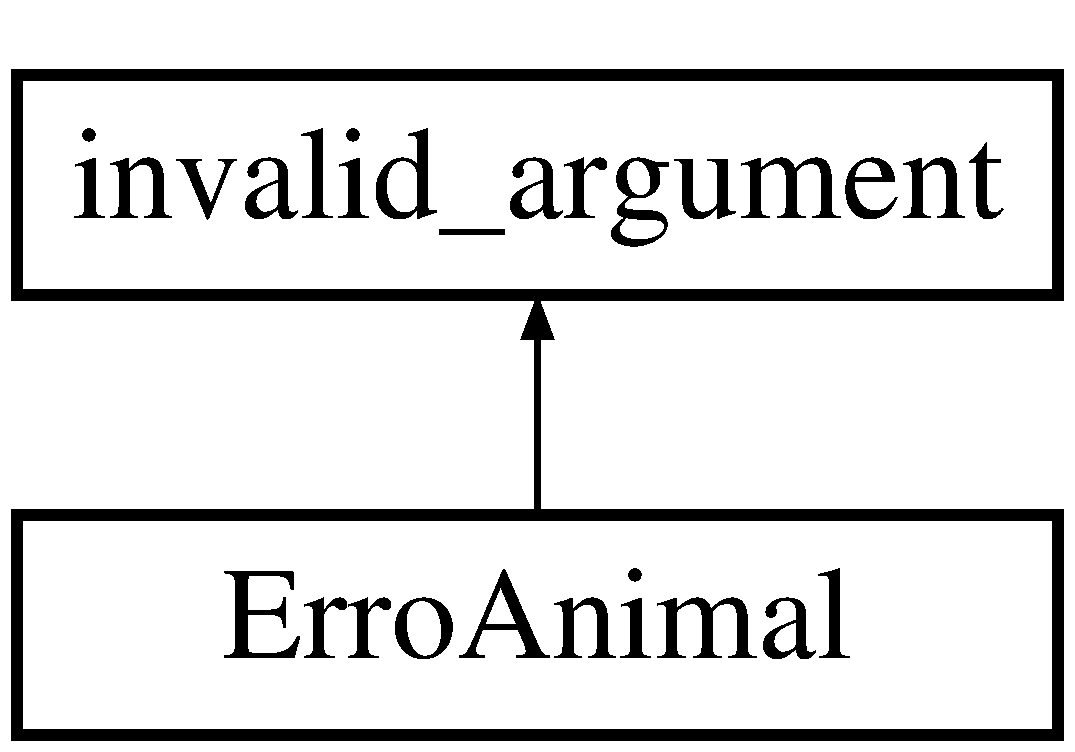
\includegraphics[height=2.000000cm]{class_erro_animal}
\end{center}
\end{figure}


\subsection{Detailed Description}
Um tratamento de excessão. 

Utilizado para quando houver um erro na chamada de um \mbox{\hyperlink{class_animal}{Animal}} 

The documentation for this class was generated from the following file\+:\begin{DoxyCompactItemize}
\item 
doxygen/menu.\+h\end{DoxyCompactItemize}

\hypertarget{class_erro_de_insercao}{}\section{Erro\+De\+Insercao Class Reference}
\label{class_erro_de_insercao}\index{Erro\+De\+Insercao@{Erro\+De\+Insercao}}


Um tratamento de excessão.  




{\ttfamily \#include $<$menu.\+h$>$}

Inheritance diagram for Erro\+De\+Insercao\+:\begin{figure}[H]
\begin{center}
\leavevmode
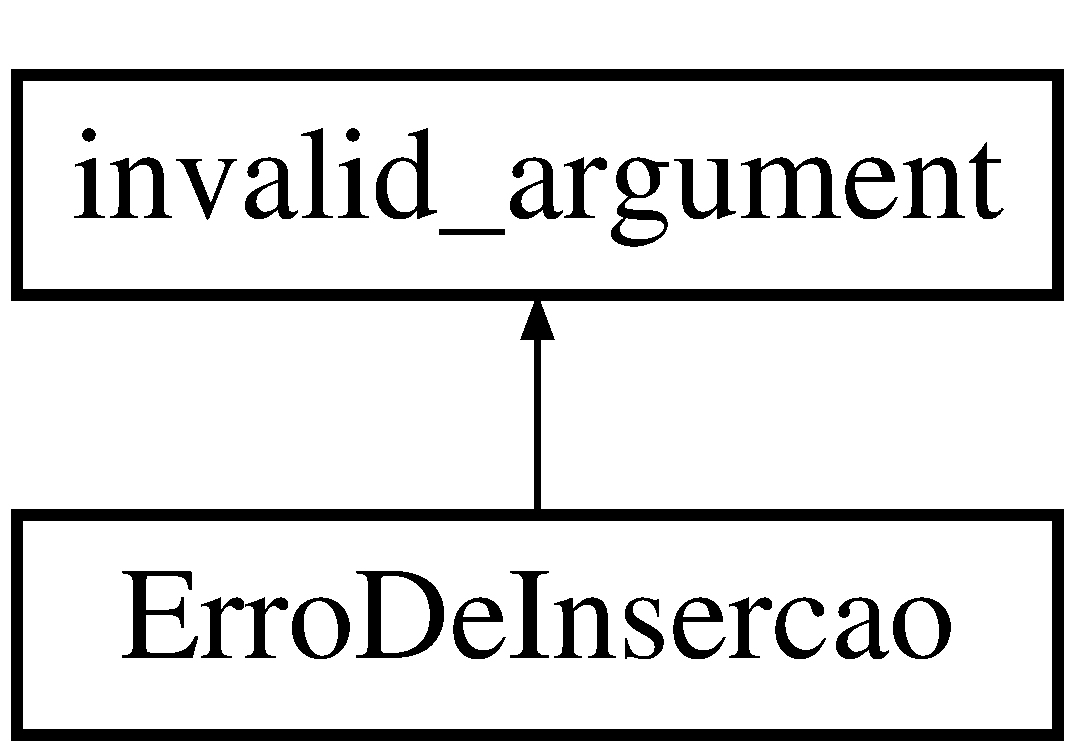
\includegraphics[height=2.000000cm]{class_erro_de_insercao}
\end{center}
\end{figure}


\subsection{Detailed Description}
Um tratamento de excessão. 

Utilizado para quando houver um erro de inserção geral 

The documentation for this class was generated from the following file\+:\begin{DoxyCompactItemize}
\item 
doxygen/menu.\+h\end{DoxyCompactItemize}

\hypertarget{class_erro_funcionario}{}\section{Erro\+Funcionario Class Reference}
\label{class_erro_funcionario}\index{Erro\+Funcionario@{Erro\+Funcionario}}


Um tratamento de excessão.  




{\ttfamily \#include $<$menu.\+h$>$}

Inheritance diagram for Erro\+Funcionario\+:\begin{figure}[H]
\begin{center}
\leavevmode
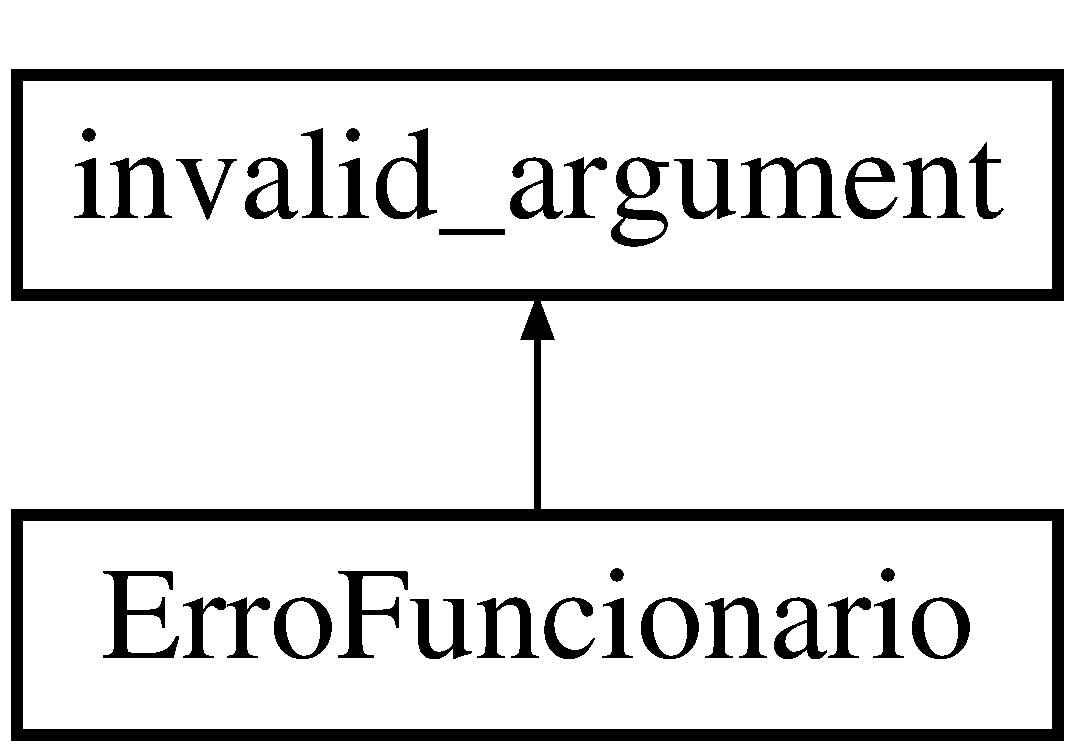
\includegraphics[height=2.000000cm]{class_erro_funcionario}
\end{center}
\end{figure}


\subsection{Detailed Description}
Um tratamento de excessão. 

Utilizado para quando houver um erro na chamada de um funcionário 

The documentation for this class was generated from the following file\+:\begin{DoxyCompactItemize}
\item 
doxygen/menu.\+h\end{DoxyCompactItemize}

\hypertarget{class_erro_id}{}\section{Erro\+Id Class Reference}
\label{class_erro_id}\index{Erro\+Id@{Erro\+Id}}


Um tratamento de excessão.  




{\ttfamily \#include $<$menu.\+h$>$}

Inheritance diagram for Erro\+Id\+:\begin{figure}[H]
\begin{center}
\leavevmode
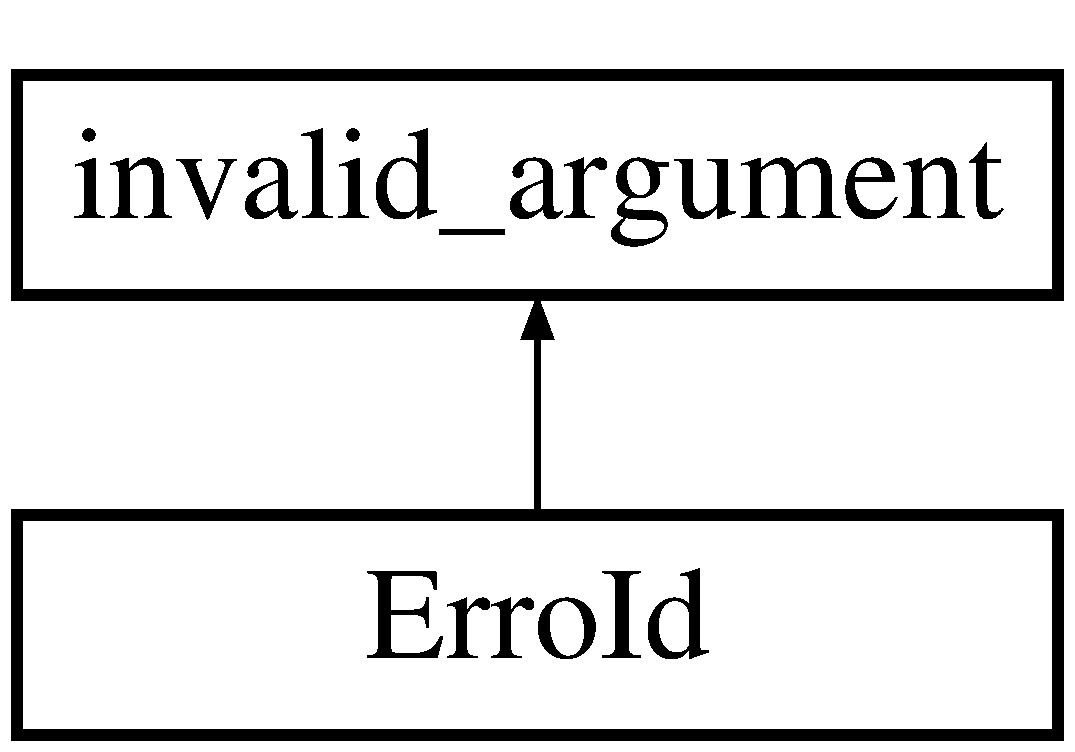
\includegraphics[height=2.000000cm]{class_erro_id}
\end{center}
\end{figure}


\subsection{Detailed Description}
Um tratamento de excessão. 

Utilizado para quando houver um erro na chamada do ID 

The documentation for this class was generated from the following file\+:\begin{DoxyCompactItemize}
\item 
doxygen/menu.\+h\end{DoxyCompactItemize}

\hypertarget{class_erro_tipo_sanguineo}{}\section{Erro\+Tipo\+Sanguineo Class Reference}
\label{class_erro_tipo_sanguineo}\index{Erro\+Tipo\+Sanguineo@{Erro\+Tipo\+Sanguineo}}


Um tratamento de excessão.  




{\ttfamily \#include $<$menu.\+h$>$}

Inheritance diagram for Erro\+Tipo\+Sanguineo\+:\begin{figure}[H]
\begin{center}
\leavevmode
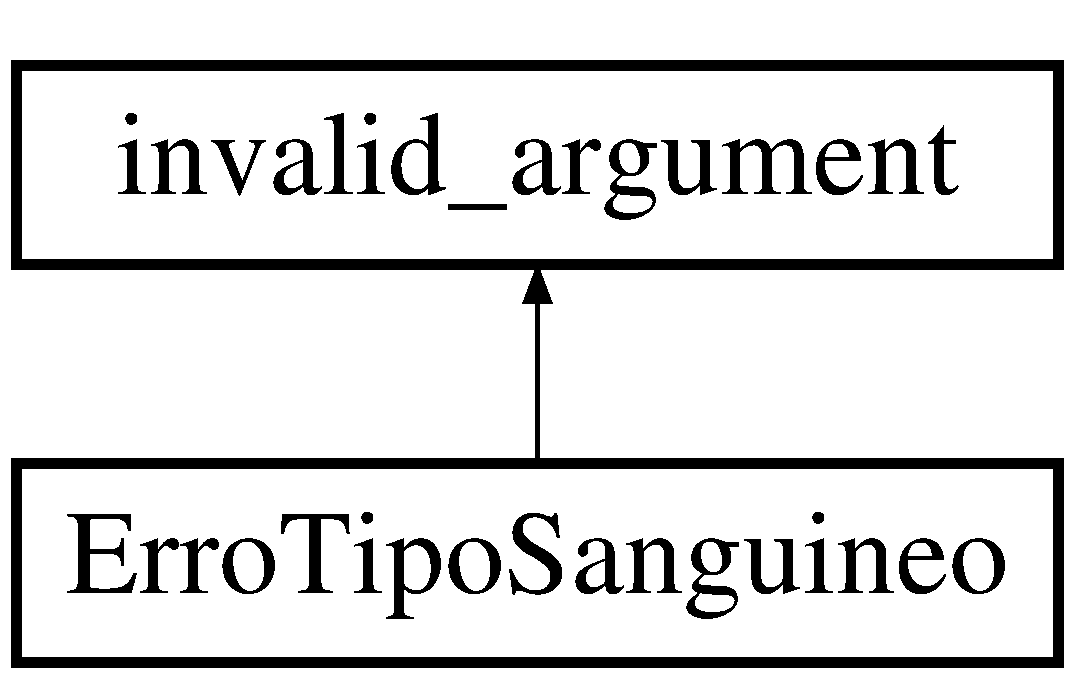
\includegraphics[height=2.000000cm]{class_erro_tipo_sanguineo}
\end{center}
\end{figure}


\subsection{Detailed Description}
Um tratamento de excessão. 

Utilizado para quando houver um erro de inserção no Tipo sanguineo 

The documentation for this class was generated from the following file\+:\begin{DoxyCompactItemize}
\item 
doxygen/menu.\+h\end{DoxyCompactItemize}

\hypertarget{classfuncionario}{}\section{funcionario Class Reference}
\label{classfuncionario}\index{funcionario@{funcionario}}


Criação da classe funcionário.  




{\ttfamily \#include $<$funcionario.\+h$>$}

Inheritance diagram for funcionario\+:\begin{figure}[H]
\begin{center}
\leavevmode
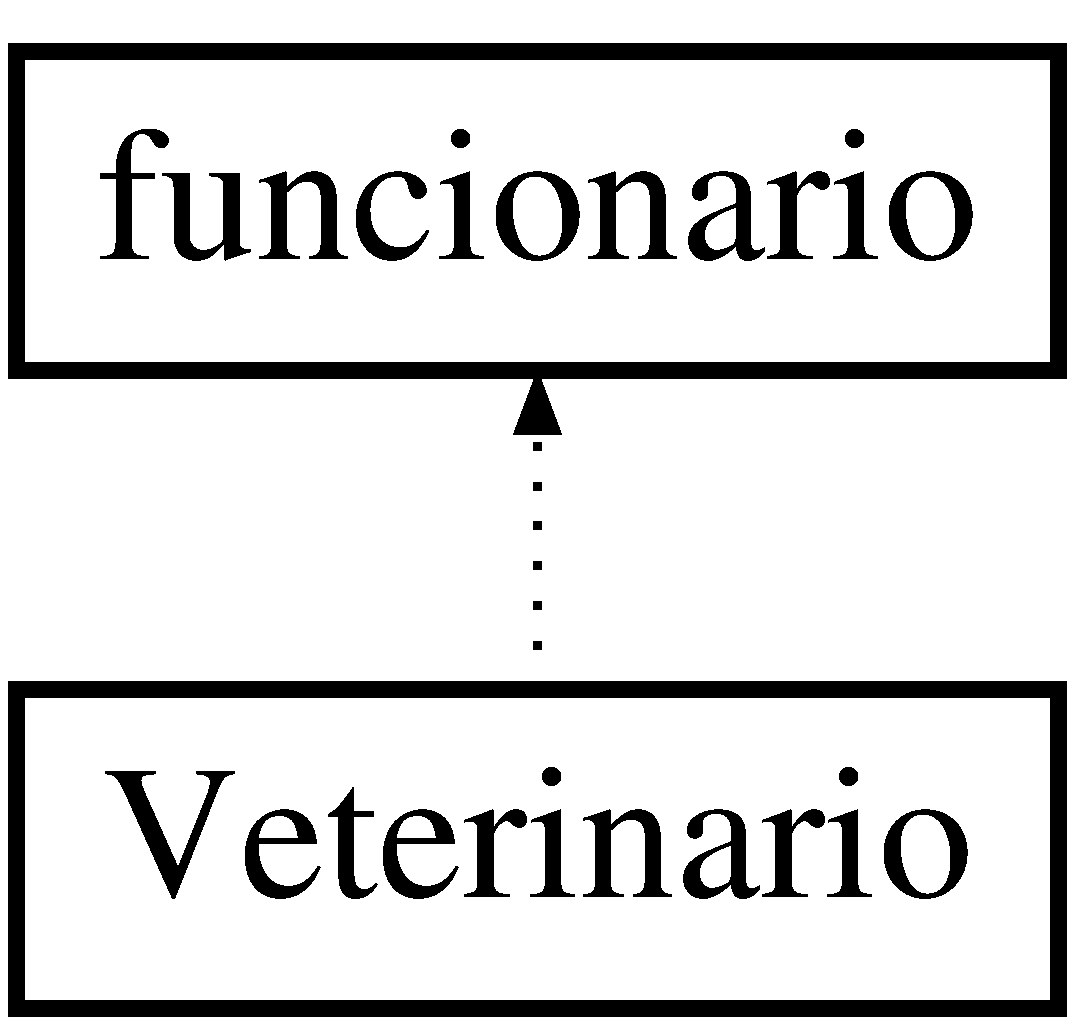
\includegraphics[height=2.000000cm]{classfuncionario}
\end{center}
\end{figure}
\subsection*{Protected Attributes}
\begin{DoxyCompactItemize}
\item 
int \mbox{\hyperlink{classfuncionario_ad48715f6be92d7cf934b0dd51c8ee42e}{id}}
\begin{DoxyCompactList}\small\item\em Criação dos parâmetros da classe funcionário. \end{DoxyCompactList}\item 
\mbox{\Hypertarget{classfuncionario_a22abef9e62c546e487df049df90cf0ef}\label{classfuncionario_a22abef9e62c546e487df049df90cf0ef}} 
string {\bfseries nome}
\item 
\mbox{\Hypertarget{classfuncionario_a25ecd173967565446dbe936ce193d702}\label{classfuncionario_a25ecd173967565446dbe936ce193d702}} 
string {\bfseries cpf}
\item 
\mbox{\Hypertarget{classfuncionario_a451f9d7e02bc1eac8255ef79daad15ba}\label{classfuncionario_a451f9d7e02bc1eac8255ef79daad15ba}} 
string {\bfseries idade}
\item 
\mbox{\Hypertarget{classfuncionario_abedbfcc85cf879c4c6d703c3a0adfb99}\label{classfuncionario_abedbfcc85cf879c4c6d703c3a0adfb99}} 
string {\bfseries tipo\+\_\+sanguineo}
\item 
\mbox{\Hypertarget{classfuncionario_a47d9fec23a2e4b83f451c4e6752e9966}\label{classfuncionario_a47d9fec23a2e4b83f451c4e6752e9966}} 
string {\bfseries fator\+RH}
\item 
\mbox{\Hypertarget{classfuncionario_a67256822db99e87eb331edac90ab19bd}\label{classfuncionario_a67256822db99e87eb331edac90ab19bd}} 
string {\bfseries especialidade}
\end{DoxyCompactItemize}


\subsection{Detailed Description}
Criação da classe funcionário. 

\subsection{Member Data Documentation}
\mbox{\Hypertarget{classfuncionario_ad48715f6be92d7cf934b0dd51c8ee42e}\label{classfuncionario_ad48715f6be92d7cf934b0dd51c8ee42e}} 
\index{funcionario@{funcionario}!id@{id}}
\index{id@{id}!funcionario@{funcionario}}
\subsubsection{\texorpdfstring{id}{id}}
{\footnotesize\ttfamily int funcionario\+::id\hspace{0.3cm}{\ttfamily [protected]}}



Criação dos parâmetros da classe funcionário. 


\begin{DoxyParams}{Parameters}
{\em int} & id serve para guardar o ID do funcionário \\
\hline
{\em string} & nome para guardar o nome \\
\hline
{\em string} & cpf para guardar o cpf \\
\hline
{\em int} & idade para guardar a idade \\
\hline
{\em string} & tipo\+\_\+sanguineo para guardar o tipo sanguineo \\
\hline
{\em string} & fator\+RH para guardar o RH \\
\hline
{\em string} & especialidade para guardar a especialidade do funcionário \\
\hline
\end{DoxyParams}


The documentation for this class was generated from the following file\+:\begin{DoxyCompactItemize}
\item 
doxygen/funcionario.\+h\end{DoxyCompactItemize}

\hypertarget{class_mamifero}{}\section{Mamifero Class Reference}
\label{class_mamifero}\index{Mamifero@{Mamifero}}


Criação da classe \mbox{\hyperlink{class_mamifero}{Mamifero}}.  




{\ttfamily \#include $<$mamifero.\+h$>$}

Inheritance diagram for Mamifero\+:\begin{figure}[H]
\begin{center}
\leavevmode
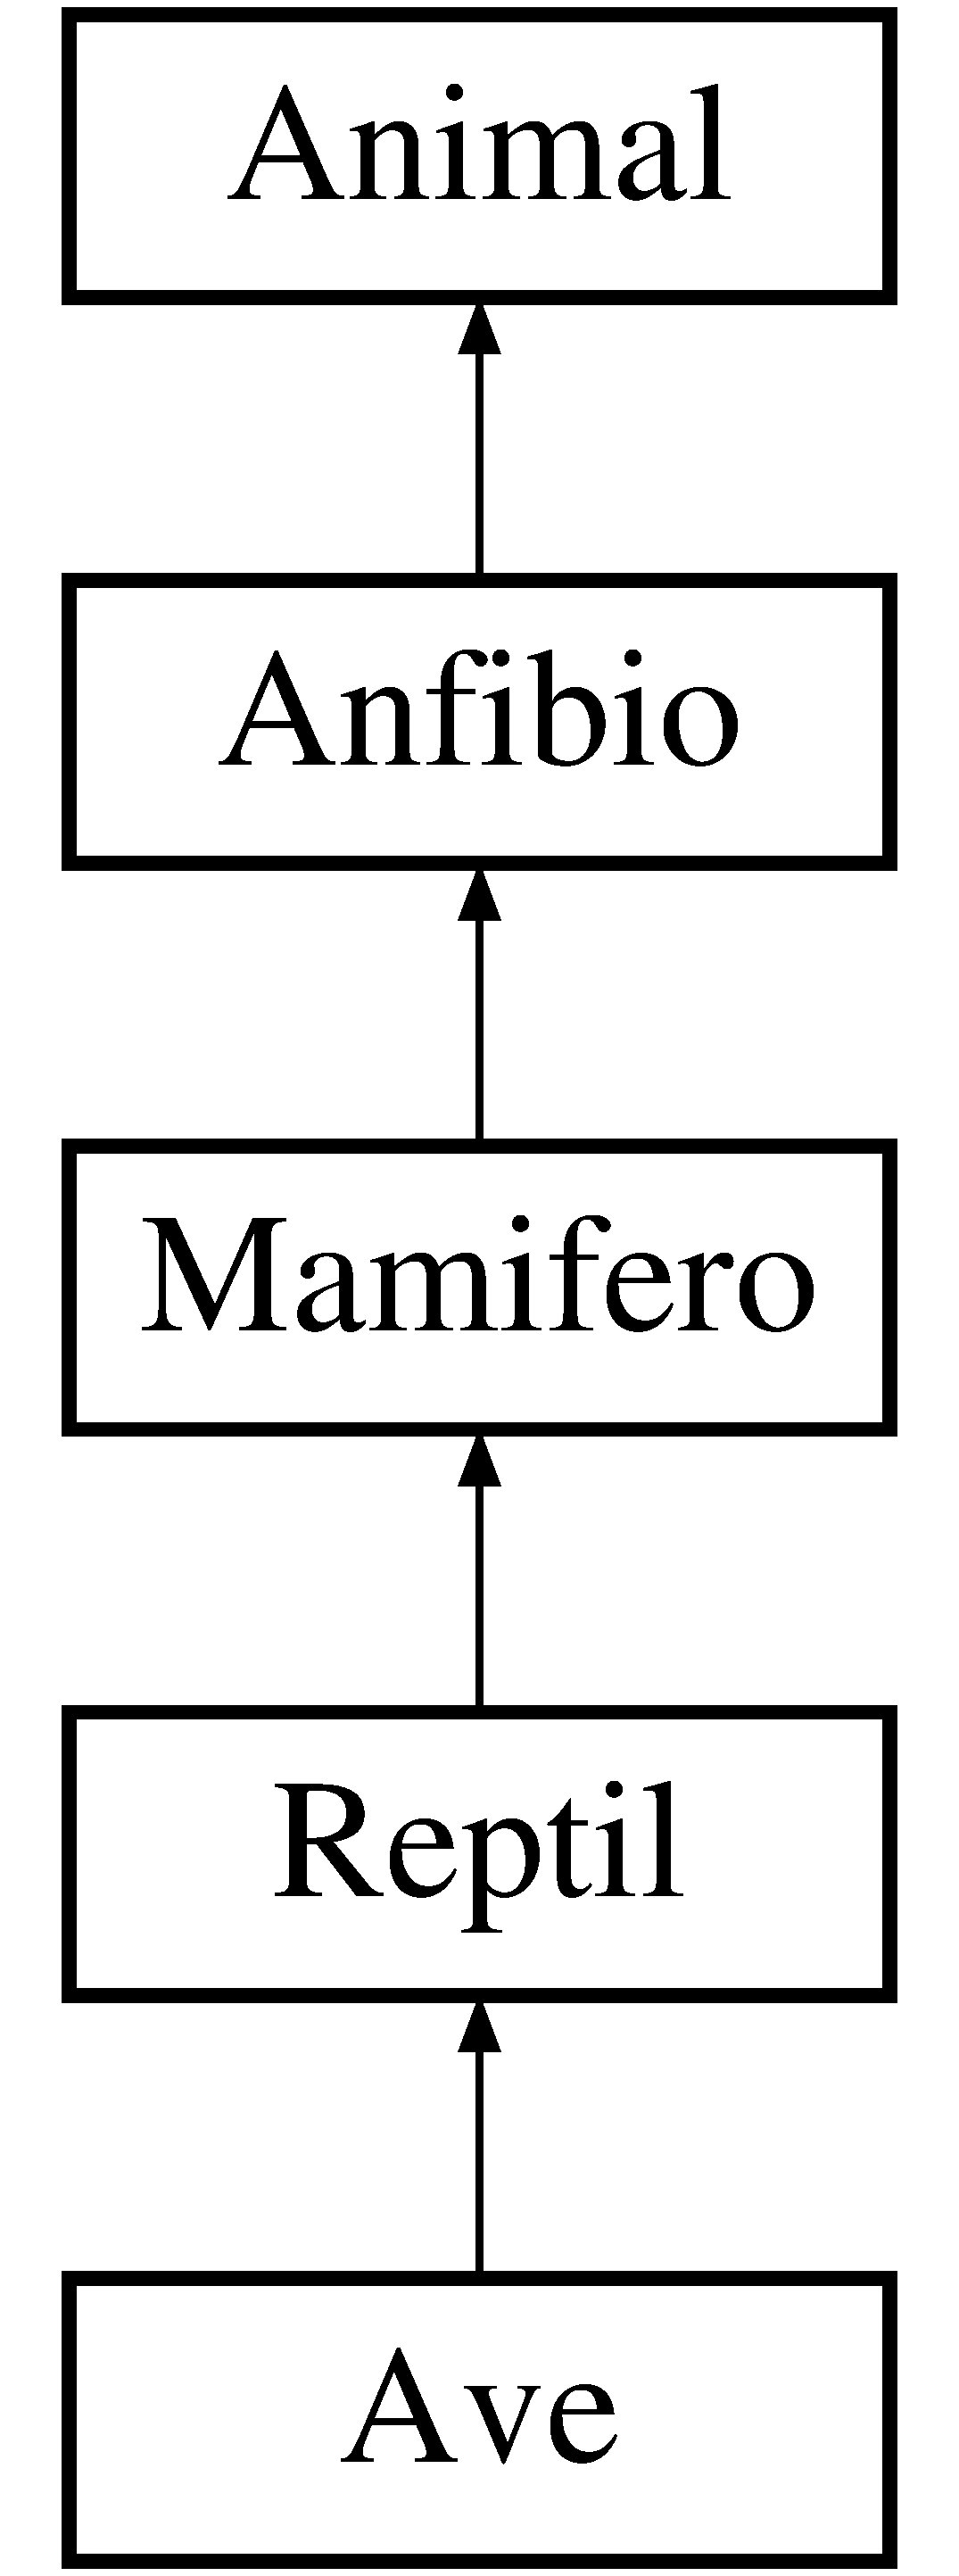
\includegraphics[height=5.000000cm]{class_mamifero}
\end{center}
\end{figure}
\subsection*{Public Member Functions}
\begin{DoxyCompactItemize}
\item 
\mbox{\hyperlink{class_mamifero_adc6af2531b40fb6b0bc91cb5bbb205e8}{Mamifero}} ()
\begin{DoxyCompactList}\small\item\em Criação do Contrutor e Destrutor. \end{DoxyCompactList}\item 
void \mbox{\hyperlink{class_mamifero_af4889c9c225884eae0f5da5db0eb9bf3}{Set\+Id}} (int id\+\_\+)
\begin{DoxyCompactList}\small\item\em Criação dos métodos Setters. \end{DoxyCompactList}\item 
\mbox{\Hypertarget{class_mamifero_ae4208a1463184117191a92dbbba14386}\label{class_mamifero_ae4208a1463184117191a92dbbba14386}} 
void \mbox{\hyperlink{class_mamifero_ae4208a1463184117191a92dbbba14386}{Set\+Classe}} (string classe\+\_\+)
\begin{DoxyCompactList}\small\item\em Chamada do metodo \mbox{\hyperlink{class_mamifero_ae4208a1463184117191a92dbbba14386}{Set\+Classe()}} \end{DoxyCompactList}\item 
\mbox{\Hypertarget{class_mamifero_a17c9d20e75ab1a92432792e99871de64}\label{class_mamifero_a17c9d20e75ab1a92432792e99871de64}} 
void \mbox{\hyperlink{class_mamifero_a17c9d20e75ab1a92432792e99871de64}{Set\+Nome}} (string nome\+\_\+)
\begin{DoxyCompactList}\small\item\em Chamada do metodo \mbox{\hyperlink{class_mamifero_a17c9d20e75ab1a92432792e99871de64}{Set\+Nome()}} \end{DoxyCompactList}\item 
\mbox{\Hypertarget{class_mamifero_a284d68ac9ac3c0cc5a08886117d7fe9b}\label{class_mamifero_a284d68ac9ac3c0cc5a08886117d7fe9b}} 
void \mbox{\hyperlink{class_mamifero_a284d68ac9ac3c0cc5a08886117d7fe9b}{Set\+Cientifico}} (string cientifico\+\_\+)
\begin{DoxyCompactList}\small\item\em Chamada do metodo \mbox{\hyperlink{class_mamifero_a284d68ac9ac3c0cc5a08886117d7fe9b}{Set\+Cientifico()}} \end{DoxyCompactList}\item 
\mbox{\Hypertarget{class_mamifero_a975d11c7244dbc2f623fbcf439eb0e05}\label{class_mamifero_a975d11c7244dbc2f623fbcf439eb0e05}} 
void \mbox{\hyperlink{class_mamifero_a975d11c7244dbc2f623fbcf439eb0e05}{Set\+Sexo}} (string sexo\+\_\+)
\begin{DoxyCompactList}\small\item\em Chamada do metodo \mbox{\hyperlink{class_mamifero_a975d11c7244dbc2f623fbcf439eb0e05}{Set\+Sexo()}} \end{DoxyCompactList}\item 
\mbox{\Hypertarget{class_mamifero_a9f1140c23345bf034a354e95d26c01ef}\label{class_mamifero_a9f1140c23345bf034a354e95d26c01ef}} 
void \mbox{\hyperlink{class_mamifero_a9f1140c23345bf034a354e95d26c01ef}{Set\+Tamanho}} (float tamanho\+\_\+)
\begin{DoxyCompactList}\small\item\em Chamada do metodo \mbox{\hyperlink{class_mamifero_a9f1140c23345bf034a354e95d26c01ef}{Set\+Tamanho()}} \end{DoxyCompactList}\item 
\mbox{\Hypertarget{class_mamifero_a75ef68575458f4de5e0e749c0794c384}\label{class_mamifero_a75ef68575458f4de5e0e749c0794c384}} 
void \mbox{\hyperlink{class_mamifero_a75ef68575458f4de5e0e749c0794c384}{Set\+Dieta}} (string dieta\+\_\+)
\begin{DoxyCompactList}\small\item\em Chamada do metodo \mbox{\hyperlink{class_mamifero_a75ef68575458f4de5e0e749c0794c384}{Set\+Dieta()}} \end{DoxyCompactList}\item 
\mbox{\Hypertarget{class_mamifero_af7f46618a26baef314e26affc4e93363}\label{class_mamifero_af7f46618a26baef314e26affc4e93363}} 
void \mbox{\hyperlink{class_mamifero_af7f46618a26baef314e26affc4e93363}{Set\+Veterinario}} (int veterinario\+\_\+)
\begin{DoxyCompactList}\small\item\em Chamada do metodo \mbox{\hyperlink{class_mamifero_af7f46618a26baef314e26affc4e93363}{Set\+Veterinario()}} \end{DoxyCompactList}\item 
\mbox{\Hypertarget{class_mamifero_a749a1745469c00afd74575f02c900573}\label{class_mamifero_a749a1745469c00afd74575f02c900573}} 
void \mbox{\hyperlink{class_mamifero_a749a1745469c00afd74575f02c900573}{Set\+Tratador}} (int tratador\+\_\+)
\begin{DoxyCompactList}\small\item\em Chamada do metodo \mbox{\hyperlink{class_mamifero_a749a1745469c00afd74575f02c900573}{Set\+Tratador()}} \end{DoxyCompactList}\item 
\mbox{\Hypertarget{class_mamifero_a25532703d9fdb32d3465988e0c202ca1}\label{class_mamifero_a25532703d9fdb32d3465988e0c202ca1}} 
void \mbox{\hyperlink{class_mamifero_a25532703d9fdb32d3465988e0c202ca1}{Set\+Batismo}} (string batismo)
\begin{DoxyCompactList}\small\item\em Chamada do metodo \mbox{\hyperlink{class_mamifero_a25532703d9fdb32d3465988e0c202ca1}{Set\+Batismo()}} \end{DoxyCompactList}\item 
\mbox{\Hypertarget{class_mamifero_a3ad7da527f6329f3eae52b05839805f1}\label{class_mamifero_a3ad7da527f6329f3eae52b05839805f1}} 
void \mbox{\hyperlink{class_mamifero_a3ad7da527f6329f3eae52b05839805f1}{Set\+Cor\+Pelo}} (string cor\+\_\+pelo\+\_\+)
\begin{DoxyCompactList}\small\item\em Chamada do metodo \mbox{\hyperlink{class_mamifero_a3ad7da527f6329f3eae52b05839805f1}{Set\+Cor\+Pelo()}} \end{DoxyCompactList}\item 
int \mbox{\hyperlink{class_mamifero_ae7433cef065a2d6b76f510efc4f3e7db}{Get\+Id}} (void)
\begin{DoxyCompactList}\small\item\em Criação dos métodos Getters. \end{DoxyCompactList}\item 
\mbox{\Hypertarget{class_mamifero_a7e075212c74fcc33cfe0ac10de5646fa}\label{class_mamifero_a7e075212c74fcc33cfe0ac10de5646fa}} 
string \mbox{\hyperlink{class_mamifero_a7e075212c74fcc33cfe0ac10de5646fa}{Get\+Classe}} (void)
\begin{DoxyCompactList}\small\item\em Chamada do metodo \mbox{\hyperlink{class_mamifero_a7e075212c74fcc33cfe0ac10de5646fa}{Get\+Classe()}} \end{DoxyCompactList}\item 
\mbox{\Hypertarget{class_mamifero_a22f2b88c72b6d1b15af4ded57a07c759}\label{class_mamifero_a22f2b88c72b6d1b15af4ded57a07c759}} 
string \mbox{\hyperlink{class_mamifero_a22f2b88c72b6d1b15af4ded57a07c759}{Get\+Nome}} (void)
\begin{DoxyCompactList}\small\item\em Chamada do metodo \mbox{\hyperlink{class_mamifero_a22f2b88c72b6d1b15af4ded57a07c759}{Get\+Nome()}} \end{DoxyCompactList}\item 
\mbox{\Hypertarget{class_mamifero_ab3a9c6cda70d78e7e870e90d30494349}\label{class_mamifero_ab3a9c6cda70d78e7e870e90d30494349}} 
string \mbox{\hyperlink{class_mamifero_ab3a9c6cda70d78e7e870e90d30494349}{Get\+Cientifico}} (void)
\begin{DoxyCompactList}\small\item\em Chamada do metodo \mbox{\hyperlink{class_mamifero_ab3a9c6cda70d78e7e870e90d30494349}{Get\+Cientifico()}} \end{DoxyCompactList}\item 
\mbox{\Hypertarget{class_mamifero_afe12f7f2be24fa0abb9ffc2d9aebc802}\label{class_mamifero_afe12f7f2be24fa0abb9ffc2d9aebc802}} 
string \mbox{\hyperlink{class_mamifero_afe12f7f2be24fa0abb9ffc2d9aebc802}{Get\+Sexo}} (void)
\begin{DoxyCompactList}\small\item\em Chamada do metodo \mbox{\hyperlink{class_mamifero_afe12f7f2be24fa0abb9ffc2d9aebc802}{Get\+Sexo()}} \end{DoxyCompactList}\item 
\mbox{\Hypertarget{class_mamifero_ad2ef734023f5c188b4ca46b3d4bb39f7}\label{class_mamifero_ad2ef734023f5c188b4ca46b3d4bb39f7}} 
float \mbox{\hyperlink{class_mamifero_ad2ef734023f5c188b4ca46b3d4bb39f7}{Get\+Tamanho}} (void)
\begin{DoxyCompactList}\small\item\em Chamada do metodo \mbox{\hyperlink{class_mamifero_ad2ef734023f5c188b4ca46b3d4bb39f7}{Get\+Tamanho()}} \end{DoxyCompactList}\item 
\mbox{\Hypertarget{class_mamifero_a774cf3110947e5a3a0ce83aaf1f385aa}\label{class_mamifero_a774cf3110947e5a3a0ce83aaf1f385aa}} 
string \mbox{\hyperlink{class_mamifero_a774cf3110947e5a3a0ce83aaf1f385aa}{Get\+Dieta}} (void)
\begin{DoxyCompactList}\small\item\em Chamada do metodo \mbox{\hyperlink{class_mamifero_a774cf3110947e5a3a0ce83aaf1f385aa}{Get\+Dieta()}} \end{DoxyCompactList}\item 
\mbox{\Hypertarget{class_mamifero_ad9b68bdf7b8ab72cfe40a6969fd0c1e3}\label{class_mamifero_ad9b68bdf7b8ab72cfe40a6969fd0c1e3}} 
int \mbox{\hyperlink{class_mamifero_ad9b68bdf7b8ab72cfe40a6969fd0c1e3}{Get\+Veterinario}} (void)
\begin{DoxyCompactList}\small\item\em Chamada do metodo \mbox{\hyperlink{class_mamifero_ad9b68bdf7b8ab72cfe40a6969fd0c1e3}{Get\+Veterinario()}} \end{DoxyCompactList}\item 
\mbox{\Hypertarget{class_mamifero_aefe8a8e19be80f7486a475b19c4d97ac}\label{class_mamifero_aefe8a8e19be80f7486a475b19c4d97ac}} 
int \mbox{\hyperlink{class_mamifero_aefe8a8e19be80f7486a475b19c4d97ac}{Get\+Tratador}} (void)
\begin{DoxyCompactList}\small\item\em Chamada do metodo \mbox{\hyperlink{class_mamifero_aefe8a8e19be80f7486a475b19c4d97ac}{Get\+Tratador()}} \end{DoxyCompactList}\item 
\mbox{\Hypertarget{class_mamifero_a0b7058dd9e9fc48082935ef0a8e4f1e8}\label{class_mamifero_a0b7058dd9e9fc48082935ef0a8e4f1e8}} 
string \mbox{\hyperlink{class_mamifero_a0b7058dd9e9fc48082935ef0a8e4f1e8}{Get\+Batismo}} (void)
\begin{DoxyCompactList}\small\item\em Chamada do metodo \mbox{\hyperlink{class_mamifero_a0b7058dd9e9fc48082935ef0a8e4f1e8}{Get\+Batismo()}} \end{DoxyCompactList}\item 
\mbox{\Hypertarget{class_mamifero_a1a10413bed9db3c6ddcd39ed55ecc7a2}\label{class_mamifero_a1a10413bed9db3c6ddcd39ed55ecc7a2}} 
string \mbox{\hyperlink{class_mamifero_a1a10413bed9db3c6ddcd39ed55ecc7a2}{Get\+Cor\+Pelo}} (void)
\begin{DoxyCompactList}\small\item\em Chamada do metodo \mbox{\hyperlink{class_mamifero_a1a10413bed9db3c6ddcd39ed55ecc7a2}{Get\+Cor\+Pelo()}} \end{DoxyCompactList}\end{DoxyCompactItemize}
\subsection*{Protected Attributes}
\begin{DoxyCompactItemize}
\item 
string \mbox{\hyperlink{class_mamifero_afa5db00bf6dcf9b2e4e4d24f6d51a36c}{cor\+\_\+pelo}}
\begin{DoxyCompactList}\small\item\em Criação dos parâmetros da classe Memifero. \end{DoxyCompactList}\end{DoxyCompactItemize}
\subsection*{Additional Inherited Members}


\subsection{Detailed Description}
Criação da classe \mbox{\hyperlink{class_mamifero}{Mamifero}}. 

A classe \mbox{\hyperlink{class_mamifero}{Mamifero}} herda os parâmetros da classe \mbox{\hyperlink{class_anfibio}{Anfibio}} 

\subsection{Constructor \& Destructor Documentation}
\mbox{\Hypertarget{class_mamifero_adc6af2531b40fb6b0bc91cb5bbb205e8}\label{class_mamifero_adc6af2531b40fb6b0bc91cb5bbb205e8}} 
\index{Mamifero@{Mamifero}!Mamifero@{Mamifero}}
\index{Mamifero@{Mamifero}!Mamifero@{Mamifero}}
\subsubsection{\texorpdfstring{Mamifero()}{Mamifero()}}
{\footnotesize\ttfamily Mamifero\+::\+Mamifero (\begin{DoxyParamCaption}{ }\end{DoxyParamCaption})}



Criação do Contrutor e Destrutor. 

Chamada do contrutor e destrutor() 

\subsection{Member Function Documentation}
\mbox{\Hypertarget{class_mamifero_ae7433cef065a2d6b76f510efc4f3e7db}\label{class_mamifero_ae7433cef065a2d6b76f510efc4f3e7db}} 
\index{Mamifero@{Mamifero}!Get\+Id@{Get\+Id}}
\index{Get\+Id@{Get\+Id}!Mamifero@{Mamifero}}
\subsubsection{\texorpdfstring{Get\+Id()}{GetId()}}
{\footnotesize\ttfamily int Mamifero\+::\+Get\+Id (\begin{DoxyParamCaption}\item[{void}]{ }\end{DoxyParamCaption})}



Criação dos métodos Getters. 

Chamada do metodo \mbox{\hyperlink{class_mamifero_ae7433cef065a2d6b76f510efc4f3e7db}{Get\+Id()}} \mbox{\Hypertarget{class_mamifero_af4889c9c225884eae0f5da5db0eb9bf3}\label{class_mamifero_af4889c9c225884eae0f5da5db0eb9bf3}} 
\index{Mamifero@{Mamifero}!Set\+Id@{Set\+Id}}
\index{Set\+Id@{Set\+Id}!Mamifero@{Mamifero}}
\subsubsection{\texorpdfstring{Set\+Id()}{SetId()}}
{\footnotesize\ttfamily void Mamifero\+::\+Set\+Id (\begin{DoxyParamCaption}\item[{int}]{id\+\_\+ }\end{DoxyParamCaption})}



Criação dos métodos Setters. 

Chamada do metodo \mbox{\hyperlink{class_mamifero_af4889c9c225884eae0f5da5db0eb9bf3}{Set\+Id()}} 

\subsection{Member Data Documentation}
\mbox{\Hypertarget{class_mamifero_afa5db00bf6dcf9b2e4e4d24f6d51a36c}\label{class_mamifero_afa5db00bf6dcf9b2e4e4d24f6d51a36c}} 
\index{Mamifero@{Mamifero}!cor\+\_\+pelo@{cor\+\_\+pelo}}
\index{cor\+\_\+pelo@{cor\+\_\+pelo}!Mamifero@{Mamifero}}
\subsubsection{\texorpdfstring{cor\+\_\+pelo}{cor\_pelo}}
{\footnotesize\ttfamily string Mamifero\+::cor\+\_\+pelo\hspace{0.3cm}{\ttfamily [protected]}}



Criação dos parâmetros da classe Memifero. 


\begin{DoxyParams}{Parameters}
{\em int} & cor\+\_\+pelo para guardar a cor do animal \\
\hline
\end{DoxyParams}


The documentation for this class was generated from the following files\+:\begin{DoxyCompactItemize}
\item 
doxygen/mamifero.\+h\item 
doxygen/mamifero.\+cpp\end{DoxyCompactItemize}

\hypertarget{class_reptil}{}\section{Reptil Class Reference}
\label{class_reptil}\index{Reptil@{Reptil}}


Criação da classe \mbox{\hyperlink{class_reptil}{Reptil}}.  




{\ttfamily \#include $<$reptil.\+h$>$}

Inheritance diagram for Reptil\+:\begin{figure}[H]
\begin{center}
\leavevmode
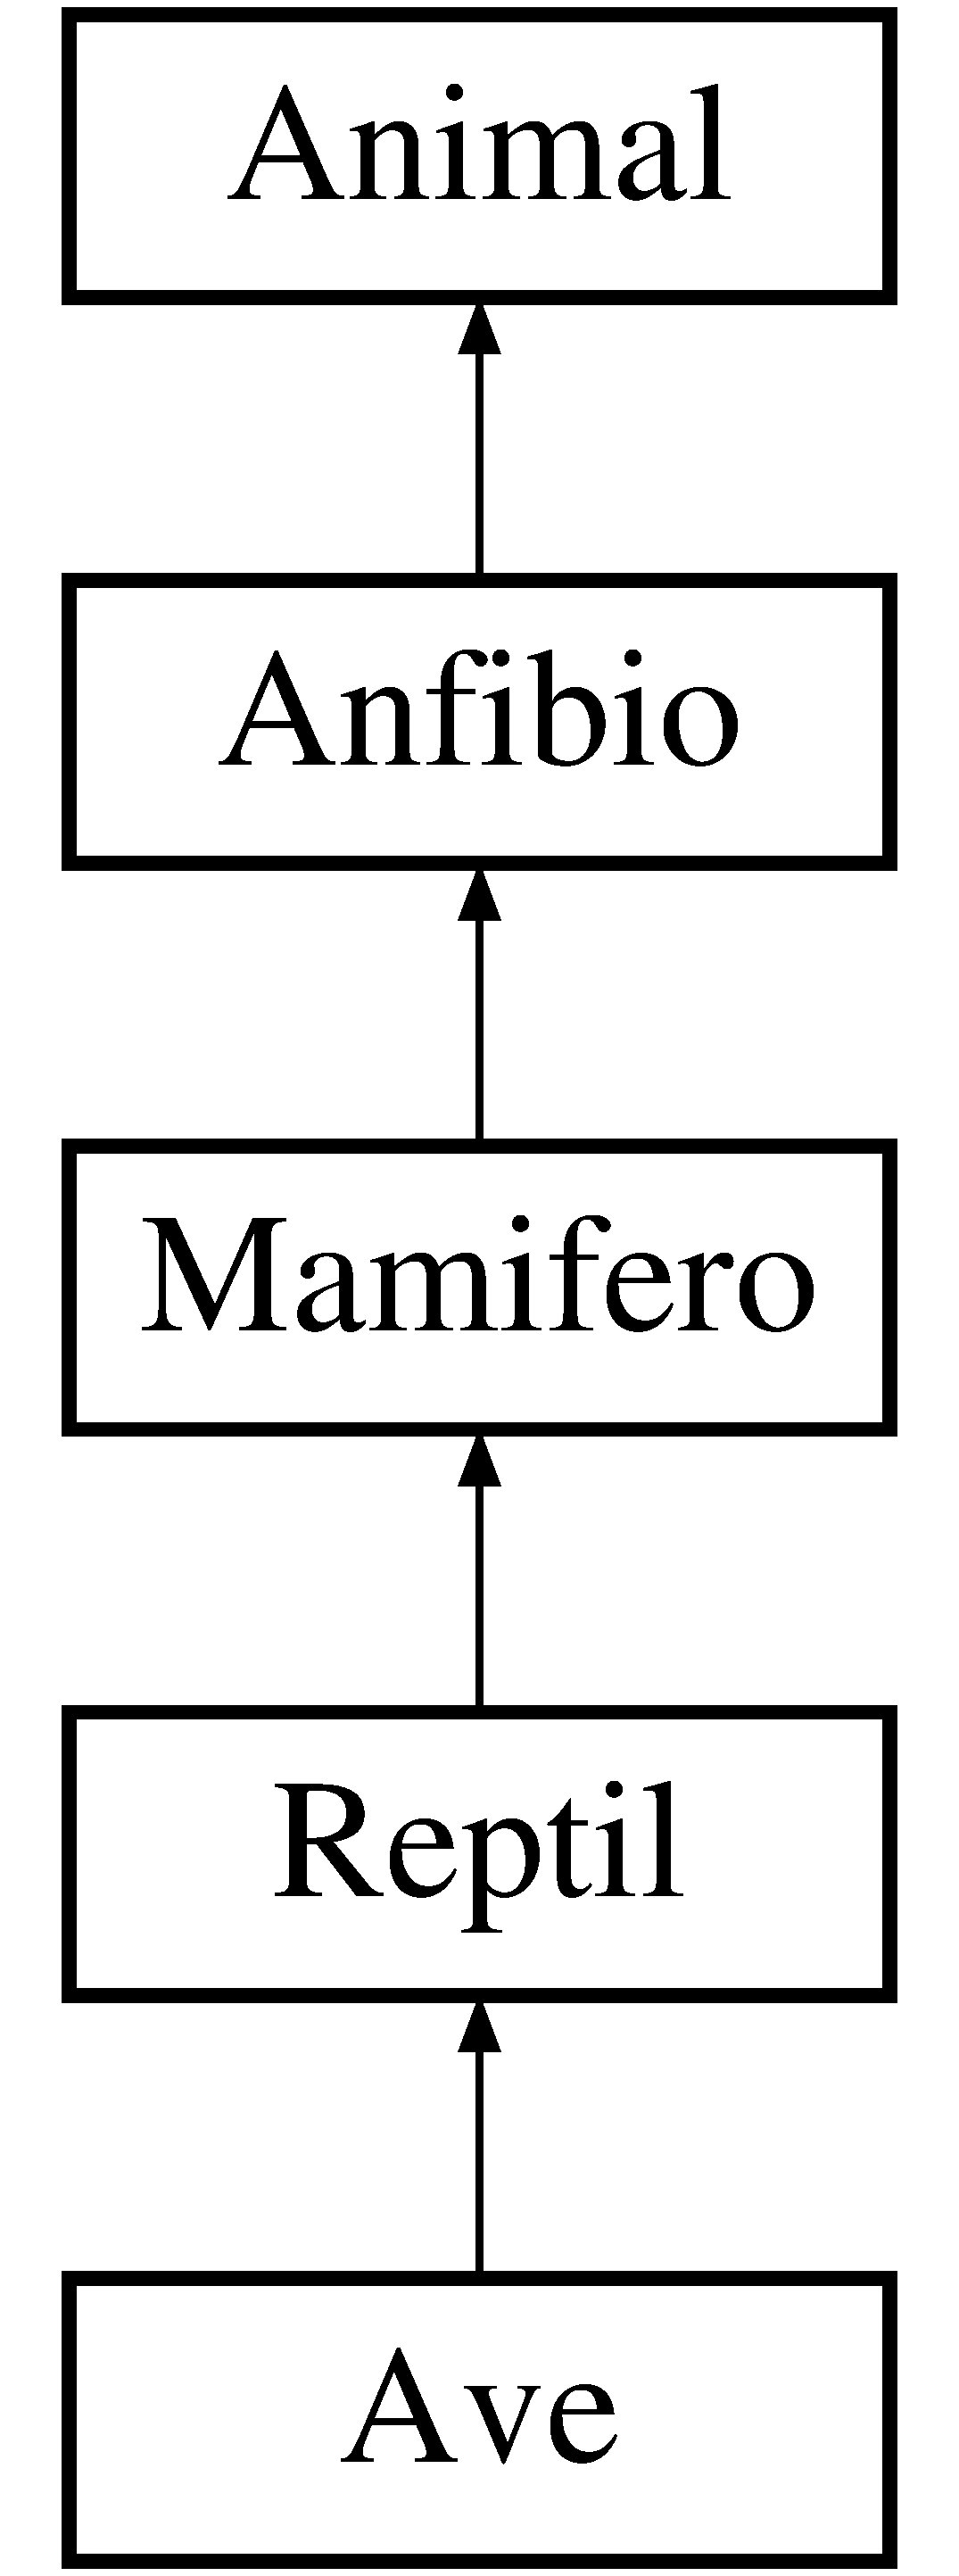
\includegraphics[height=5.000000cm]{class_reptil}
\end{center}
\end{figure}
\subsection*{Public Member Functions}
\begin{DoxyCompactItemize}
\item 
\mbox{\hyperlink{class_reptil_a8d4e391e335678b7ed64eda95e050553}{Reptil}} ()
\begin{DoxyCompactList}\small\item\em Criação do Contrutor e Destrutor. \end{DoxyCompactList}\item 
void \mbox{\hyperlink{class_reptil_a423a8162894755b69a63eefd91ba97a4}{Set\+Id}} (int id\+\_\+)
\begin{DoxyCompactList}\small\item\em Criação dos métodos Setters. \end{DoxyCompactList}\item 
\mbox{\Hypertarget{class_reptil_a2bc2e371c5a2ff4a8caddddb2015621c}\label{class_reptil_a2bc2e371c5a2ff4a8caddddb2015621c}} 
void \mbox{\hyperlink{class_reptil_a2bc2e371c5a2ff4a8caddddb2015621c}{Set\+Classe}} (string classe\+\_\+)
\begin{DoxyCompactList}\small\item\em Chamada do metodo \mbox{\hyperlink{class_reptil_a2bc2e371c5a2ff4a8caddddb2015621c}{Set\+Classe()}} \end{DoxyCompactList}\item 
\mbox{\Hypertarget{class_reptil_accbaa131894ade6bc1a4c7ad5f7b2a48}\label{class_reptil_accbaa131894ade6bc1a4c7ad5f7b2a48}} 
void \mbox{\hyperlink{class_reptil_accbaa131894ade6bc1a4c7ad5f7b2a48}{Set\+Nome}} (string nome\+\_\+)
\begin{DoxyCompactList}\small\item\em Chamada do metodo \mbox{\hyperlink{class_reptil_accbaa131894ade6bc1a4c7ad5f7b2a48}{Set\+Nome()}} \end{DoxyCompactList}\item 
\mbox{\Hypertarget{class_reptil_a006cddf27b96025050a97489b3da023b}\label{class_reptil_a006cddf27b96025050a97489b3da023b}} 
void \mbox{\hyperlink{class_reptil_a006cddf27b96025050a97489b3da023b}{Set\+Cientifico}} (string cientifico\+\_\+)
\begin{DoxyCompactList}\small\item\em Chamada do metodo \mbox{\hyperlink{class_reptil_a006cddf27b96025050a97489b3da023b}{Set\+Cientifico()}} \end{DoxyCompactList}\item 
\mbox{\Hypertarget{class_reptil_ac4d479c283df91b3e314aaf31ee37be5}\label{class_reptil_ac4d479c283df91b3e314aaf31ee37be5}} 
void \mbox{\hyperlink{class_reptil_ac4d479c283df91b3e314aaf31ee37be5}{Set\+Sexo}} (string sexo\+\_\+)
\begin{DoxyCompactList}\small\item\em Chamada do metodo \mbox{\hyperlink{class_reptil_ac4d479c283df91b3e314aaf31ee37be5}{Set\+Sexo()}} \end{DoxyCompactList}\item 
\mbox{\Hypertarget{class_reptil_a4e05aa53a93106b223811a39fb5827ee}\label{class_reptil_a4e05aa53a93106b223811a39fb5827ee}} 
void \mbox{\hyperlink{class_reptil_a4e05aa53a93106b223811a39fb5827ee}{Set\+Tamanho}} (float tamanho\+\_\+)
\begin{DoxyCompactList}\small\item\em Chamada do metodo \mbox{\hyperlink{class_reptil_a4e05aa53a93106b223811a39fb5827ee}{Set\+Tamanho()}} \end{DoxyCompactList}\item 
\mbox{\Hypertarget{class_reptil_a6d6e01ef1c8b79ad11ab9ff3b8e5f3af}\label{class_reptil_a6d6e01ef1c8b79ad11ab9ff3b8e5f3af}} 
void \mbox{\hyperlink{class_reptil_a6d6e01ef1c8b79ad11ab9ff3b8e5f3af}{Set\+Dieta}} (string dieta\+\_\+)
\begin{DoxyCompactList}\small\item\em Chamada do metodo \mbox{\hyperlink{class_reptil_a6d6e01ef1c8b79ad11ab9ff3b8e5f3af}{Set\+Dieta()}} \end{DoxyCompactList}\item 
\mbox{\Hypertarget{class_reptil_a279316a914385dee8fe1a1ff0c311162}\label{class_reptil_a279316a914385dee8fe1a1ff0c311162}} 
void \mbox{\hyperlink{class_reptil_a279316a914385dee8fe1a1ff0c311162}{Set\+Veterinario}} (int veterinario\+\_\+)
\begin{DoxyCompactList}\small\item\em Chamada do metodo \mbox{\hyperlink{class_reptil_a279316a914385dee8fe1a1ff0c311162}{Set\+Veterinario()}} \end{DoxyCompactList}\item 
\mbox{\Hypertarget{class_reptil_ae6748d6773c05db1811f72cf4fff3c3c}\label{class_reptil_ae6748d6773c05db1811f72cf4fff3c3c}} 
void \mbox{\hyperlink{class_reptil_ae6748d6773c05db1811f72cf4fff3c3c}{Set\+Tratador}} (int tratador\+\_\+)
\begin{DoxyCompactList}\small\item\em Chamada do metodo \mbox{\hyperlink{class_reptil_ae6748d6773c05db1811f72cf4fff3c3c}{Set\+Tratador()}} \end{DoxyCompactList}\item 
\mbox{\Hypertarget{class_reptil_adb957fc6ae3d2f880df6ca7dc489c93e}\label{class_reptil_adb957fc6ae3d2f880df6ca7dc489c93e}} 
void \mbox{\hyperlink{class_reptil_adb957fc6ae3d2f880df6ca7dc489c93e}{Set\+Batismo}} (string batismo)
\begin{DoxyCompactList}\small\item\em Chamada do metodo \mbox{\hyperlink{class_reptil_adb957fc6ae3d2f880df6ca7dc489c93e}{Set\+Batismo()}} \end{DoxyCompactList}\item 
\mbox{\Hypertarget{class_reptil_a761a48494eec660b0d7c72bd7b9d8aea}\label{class_reptil_a761a48494eec660b0d7c72bd7b9d8aea}} 
void \mbox{\hyperlink{class_reptil_a761a48494eec660b0d7c72bd7b9d8aea}{Set\+Venenoso}} (int venenoso\+\_\+)
\begin{DoxyCompactList}\small\item\em Chamada do metodo \mbox{\hyperlink{class_reptil_a761a48494eec660b0d7c72bd7b9d8aea}{Set\+Venenoso()}} \end{DoxyCompactList}\item 
\mbox{\Hypertarget{class_reptil_a192f9f19598d9940f4615b99d76e8aa7}\label{class_reptil_a192f9f19598d9940f4615b99d76e8aa7}} 
void \mbox{\hyperlink{class_reptil_a192f9f19598d9940f4615b99d76e8aa7}{Set\+Tipo\+Veneno}} (string veneno\+\_\+)
\begin{DoxyCompactList}\small\item\em Chamada do metodo \mbox{\hyperlink{class_reptil_a192f9f19598d9940f4615b99d76e8aa7}{Set\+Tipo\+Veneno()}} \end{DoxyCompactList}\item 
int \mbox{\hyperlink{class_reptil_af94ef2eb8b24f8751ed83a5f9786684a}{Get\+Id}} (void)
\begin{DoxyCompactList}\small\item\em Criação dos métodos Getters. \end{DoxyCompactList}\item 
\mbox{\Hypertarget{class_reptil_ad69152a0fc23d1ee082eeb452e25f8ef}\label{class_reptil_ad69152a0fc23d1ee082eeb452e25f8ef}} 
string \mbox{\hyperlink{class_reptil_ad69152a0fc23d1ee082eeb452e25f8ef}{Get\+Classe}} (void)
\begin{DoxyCompactList}\small\item\em Chamada do metodo \mbox{\hyperlink{class_reptil_ad69152a0fc23d1ee082eeb452e25f8ef}{Get\+Classe()}} \end{DoxyCompactList}\item 
\mbox{\Hypertarget{class_reptil_a0d2e760162e67653506bd3cbfc1b930f}\label{class_reptil_a0d2e760162e67653506bd3cbfc1b930f}} 
string \mbox{\hyperlink{class_reptil_a0d2e760162e67653506bd3cbfc1b930f}{Get\+Nome}} (void)
\begin{DoxyCompactList}\small\item\em Chamada do metodo \mbox{\hyperlink{class_reptil_a0d2e760162e67653506bd3cbfc1b930f}{Get\+Nome()}} \end{DoxyCompactList}\item 
\mbox{\Hypertarget{class_reptil_a1aba7e245ab718875a7efe3751825671}\label{class_reptil_a1aba7e245ab718875a7efe3751825671}} 
string \mbox{\hyperlink{class_reptil_a1aba7e245ab718875a7efe3751825671}{Get\+Cientifico}} (void)
\begin{DoxyCompactList}\small\item\em Chamada do metodo \mbox{\hyperlink{class_reptil_a1aba7e245ab718875a7efe3751825671}{Get\+Cientifico()}} \end{DoxyCompactList}\item 
\mbox{\Hypertarget{class_reptil_abcf95fc720cd1366ba40cd5d5c6b8528}\label{class_reptil_abcf95fc720cd1366ba40cd5d5c6b8528}} 
string \mbox{\hyperlink{class_reptil_abcf95fc720cd1366ba40cd5d5c6b8528}{Get\+Sexo}} (void)
\begin{DoxyCompactList}\small\item\em Chamada do metodo \mbox{\hyperlink{class_reptil_abcf95fc720cd1366ba40cd5d5c6b8528}{Get\+Sexo()}} \end{DoxyCompactList}\item 
\mbox{\Hypertarget{class_reptil_af6b79c8d921fdfe5dc5e894baeec2b25}\label{class_reptil_af6b79c8d921fdfe5dc5e894baeec2b25}} 
float \mbox{\hyperlink{class_reptil_af6b79c8d921fdfe5dc5e894baeec2b25}{Get\+Tamanho}} (void)
\begin{DoxyCompactList}\small\item\em Chamada do metodo \mbox{\hyperlink{class_reptil_af6b79c8d921fdfe5dc5e894baeec2b25}{Get\+Tamanho()}} \end{DoxyCompactList}\item 
\mbox{\Hypertarget{class_reptil_a76798ccf7c76de9cf3c17a4ce92dfd41}\label{class_reptil_a76798ccf7c76de9cf3c17a4ce92dfd41}} 
string \mbox{\hyperlink{class_reptil_a76798ccf7c76de9cf3c17a4ce92dfd41}{Get\+Dieta}} (void)
\begin{DoxyCompactList}\small\item\em Chamada do metodo \mbox{\hyperlink{class_reptil_a76798ccf7c76de9cf3c17a4ce92dfd41}{Get\+Dieta()}} \end{DoxyCompactList}\item 
\mbox{\Hypertarget{class_reptil_a41e51f10fb19549fbbf667c20adfc19f}\label{class_reptil_a41e51f10fb19549fbbf667c20adfc19f}} 
int \mbox{\hyperlink{class_reptil_a41e51f10fb19549fbbf667c20adfc19f}{Get\+Veterinario}} (void)
\begin{DoxyCompactList}\small\item\em Chamada do metodo \mbox{\hyperlink{class_reptil_a41e51f10fb19549fbbf667c20adfc19f}{Get\+Veterinario()}} \end{DoxyCompactList}\item 
\mbox{\Hypertarget{class_reptil_aa944480277a1a038f7054fdc3bd649df}\label{class_reptil_aa944480277a1a038f7054fdc3bd649df}} 
int \mbox{\hyperlink{class_reptil_aa944480277a1a038f7054fdc3bd649df}{Get\+Tratador}} (void)
\begin{DoxyCompactList}\small\item\em Chamada do metodo \mbox{\hyperlink{class_reptil_aa944480277a1a038f7054fdc3bd649df}{Get\+Tratador()}} \end{DoxyCompactList}\item 
\mbox{\Hypertarget{class_reptil_ad95008c8ec8acb80e632811eb08c3bdc}\label{class_reptil_ad95008c8ec8acb80e632811eb08c3bdc}} 
string \mbox{\hyperlink{class_reptil_ad95008c8ec8acb80e632811eb08c3bdc}{Get\+Batismo}} (void)
\begin{DoxyCompactList}\small\item\em Chamada do metodo \mbox{\hyperlink{class_reptil_ad95008c8ec8acb80e632811eb08c3bdc}{Get\+Batismo()}} \end{DoxyCompactList}\item 
\mbox{\Hypertarget{class_reptil_ad2b4e6c613913b4ba4f6a09ad9b3885e}\label{class_reptil_ad2b4e6c613913b4ba4f6a09ad9b3885e}} 
int \mbox{\hyperlink{class_reptil_ad2b4e6c613913b4ba4f6a09ad9b3885e}{Get\+Venenoso}} (void)
\begin{DoxyCompactList}\small\item\em Chamada do metodo \mbox{\hyperlink{class_reptil_ad2b4e6c613913b4ba4f6a09ad9b3885e}{Get\+Venenoso()}} \end{DoxyCompactList}\item 
\mbox{\Hypertarget{class_reptil_a8a58a42247c9ae9304e5f0d5dce72513}\label{class_reptil_a8a58a42247c9ae9304e5f0d5dce72513}} 
string \mbox{\hyperlink{class_reptil_a8a58a42247c9ae9304e5f0d5dce72513}{Get\+Tipo\+Veneno}} (void)
\begin{DoxyCompactList}\small\item\em Chamada do metodo \mbox{\hyperlink{class_reptil_a8a58a42247c9ae9304e5f0d5dce72513}{Get\+Tipo\+Veneno()}} \end{DoxyCompactList}\end{DoxyCompactItemize}
\subsection*{Protected Attributes}
\begin{DoxyCompactItemize}
\item 
int \mbox{\hyperlink{class_reptil_ac194e65b0de8ab94dd6ce75e889ba8a8}{venenoso}}
\begin{DoxyCompactList}\small\item\em Criação dos parâmetros da classe \mbox{\hyperlink{class_reptil}{Reptil}}. \end{DoxyCompactList}\item 
\mbox{\Hypertarget{class_reptil_a231d711a23c8b52ffafc135eca7a080c}\label{class_reptil_a231d711a23c8b52ffafc135eca7a080c}} 
string {\bfseries tipo\+\_\+veneno}
\end{DoxyCompactItemize}
\subsection*{Additional Inherited Members}


\subsection{Detailed Description}
Criação da classe \mbox{\hyperlink{class_reptil}{Reptil}}. 

A classe \mbox{\hyperlink{class_reptil}{Reptil}} herda os parâmetros da classe Memifero 

\subsection{Constructor \& Destructor Documentation}
\mbox{\Hypertarget{class_reptil_a8d4e391e335678b7ed64eda95e050553}\label{class_reptil_a8d4e391e335678b7ed64eda95e050553}} 
\index{Reptil@{Reptil}!Reptil@{Reptil}}
\index{Reptil@{Reptil}!Reptil@{Reptil}}
\subsubsection{\texorpdfstring{Reptil()}{Reptil()}}
{\footnotesize\ttfamily Reptil\+::\+Reptil (\begin{DoxyParamCaption}{ }\end{DoxyParamCaption})}



Criação do Contrutor e Destrutor. 

Chamada do contrutor e destrutor() 

\subsection{Member Function Documentation}
\mbox{\Hypertarget{class_reptil_af94ef2eb8b24f8751ed83a5f9786684a}\label{class_reptil_af94ef2eb8b24f8751ed83a5f9786684a}} 
\index{Reptil@{Reptil}!Get\+Id@{Get\+Id}}
\index{Get\+Id@{Get\+Id}!Reptil@{Reptil}}
\subsubsection{\texorpdfstring{Get\+Id()}{GetId()}}
{\footnotesize\ttfamily int Reptil\+::\+Get\+Id (\begin{DoxyParamCaption}\item[{void}]{ }\end{DoxyParamCaption})}



Criação dos métodos Getters. 

Chamada do metodo \mbox{\hyperlink{class_reptil_af94ef2eb8b24f8751ed83a5f9786684a}{Get\+Id()}} \mbox{\Hypertarget{class_reptil_a423a8162894755b69a63eefd91ba97a4}\label{class_reptil_a423a8162894755b69a63eefd91ba97a4}} 
\index{Reptil@{Reptil}!Set\+Id@{Set\+Id}}
\index{Set\+Id@{Set\+Id}!Reptil@{Reptil}}
\subsubsection{\texorpdfstring{Set\+Id()}{SetId()}}
{\footnotesize\ttfamily void Reptil\+::\+Set\+Id (\begin{DoxyParamCaption}\item[{int}]{id\+\_\+ }\end{DoxyParamCaption})}



Criação dos métodos Setters. 

Chamada do metodo \mbox{\hyperlink{class_reptil_a423a8162894755b69a63eefd91ba97a4}{Set\+Id()}} 

\subsection{Member Data Documentation}
\mbox{\Hypertarget{class_reptil_ac194e65b0de8ab94dd6ce75e889ba8a8}\label{class_reptil_ac194e65b0de8ab94dd6ce75e889ba8a8}} 
\index{Reptil@{Reptil}!venenoso@{venenoso}}
\index{venenoso@{venenoso}!Reptil@{Reptil}}
\subsubsection{\texorpdfstring{venenoso}{venenoso}}
{\footnotesize\ttfamily int Reptil\+::venenoso\hspace{0.3cm}{\ttfamily [protected]}}



Criação dos parâmetros da classe \mbox{\hyperlink{class_reptil}{Reptil}}. 


\begin{DoxyParams}{Parameters}
{\em int} & venenoso para guardar se o animal é venenoso ou não \\
\hline
{\em string} & tipo\+\_\+veneno para guardar o tipo do veneno \\
\hline
\end{DoxyParams}


The documentation for this class was generated from the following files\+:\begin{DoxyCompactItemize}
\item 
doxygen/reptil.\+h\item 
doxygen/reptil.\+cpp\end{DoxyCompactItemize}

\hypertarget{class_veterinario}{}\section{Veterinario Class Reference}
\label{class_veterinario}\index{Veterinario@{Veterinario}}


Criação da classe \mbox{\hyperlink{class_veterinario}{Veterinario}}.  




{\ttfamily \#include $<$veterinario.\+h$>$}

Inheritance diagram for Veterinario\+:\begin{figure}[H]
\begin{center}
\leavevmode
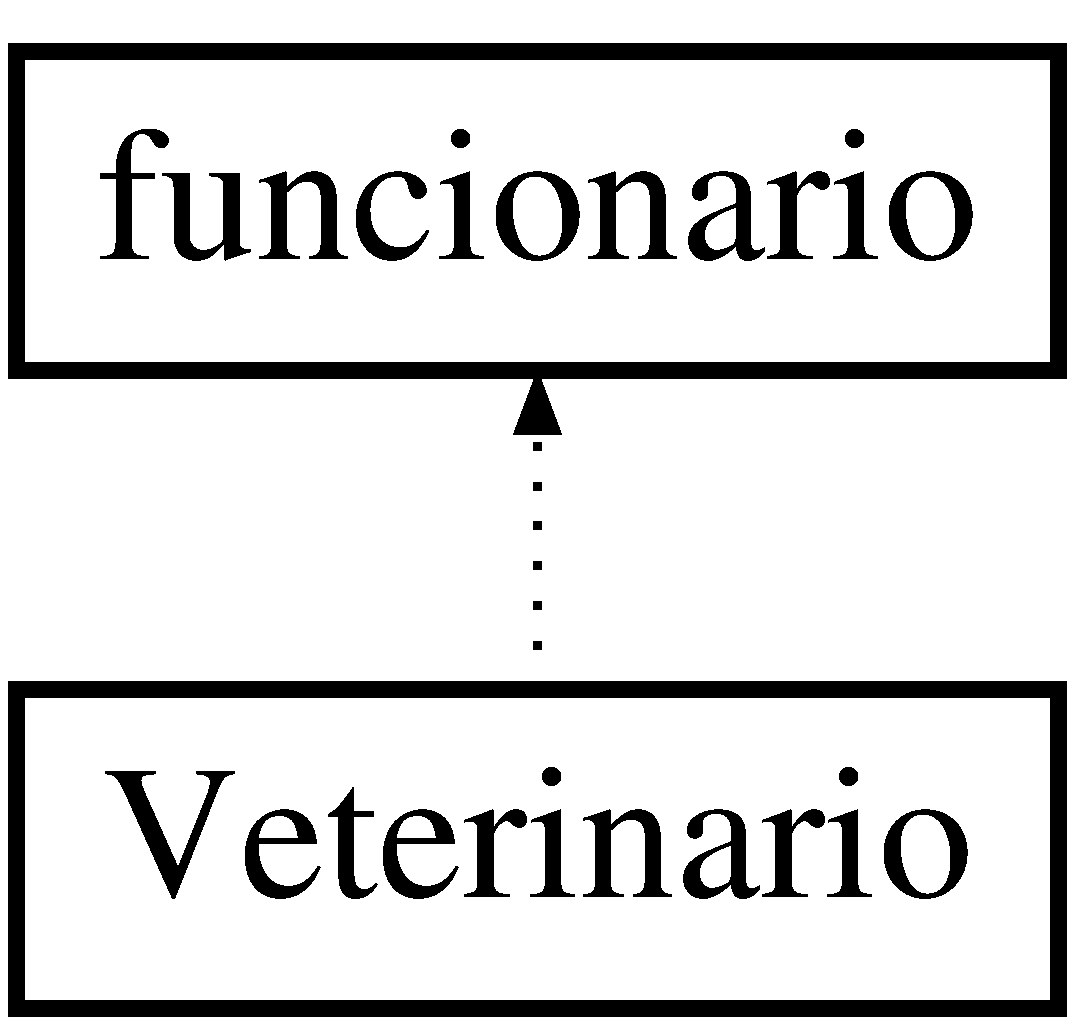
\includegraphics[height=2.000000cm]{class_veterinario}
\end{center}
\end{figure}
\subsection*{Public Member Functions}
\begin{DoxyCompactItemize}
\item 
void \mbox{\hyperlink{class_veterinario_a1852e86bed8b254e2f9b49add597b5fb}{Set\+Id}} (int id\+\_\+)
\begin{DoxyCompactList}\small\item\em Criação dos métodos Setters. \end{DoxyCompactList}\item 
\mbox{\Hypertarget{class_veterinario_a68be9e5f7903d1c3683e91ec3e4ea272}\label{class_veterinario_a68be9e5f7903d1c3683e91ec3e4ea272}} 
void \mbox{\hyperlink{class_veterinario_a68be9e5f7903d1c3683e91ec3e4ea272}{Set\+Profissao}} (string profissao\+\_\+)
\begin{DoxyCompactList}\small\item\em Chamada do metodo \mbox{\hyperlink{class_veterinario_a68be9e5f7903d1c3683e91ec3e4ea272}{Set\+Profissao()}} \end{DoxyCompactList}\item 
\mbox{\Hypertarget{class_veterinario_a4e153e6b5d2c869ace39958d69b9fa96}\label{class_veterinario_a4e153e6b5d2c869ace39958d69b9fa96}} 
void \mbox{\hyperlink{class_veterinario_a4e153e6b5d2c869ace39958d69b9fa96}{Set\+Nome}} (string nome\+\_\+)
\begin{DoxyCompactList}\small\item\em Chamada do metodo \mbox{\hyperlink{class_veterinario_a4e153e6b5d2c869ace39958d69b9fa96}{Set\+Nome()}} \end{DoxyCompactList}\item 
\mbox{\Hypertarget{class_veterinario_a3d534f523d35ed98dfd86498a2cdb59b}\label{class_veterinario_a3d534f523d35ed98dfd86498a2cdb59b}} 
void \mbox{\hyperlink{class_veterinario_a3d534f523d35ed98dfd86498a2cdb59b}{Set\+C\+PF}} (string cpf\+\_\+)
\begin{DoxyCompactList}\small\item\em Chamada do metodo \mbox{\hyperlink{class_veterinario_a3d534f523d35ed98dfd86498a2cdb59b}{Set\+C\+P\+F()}} \end{DoxyCompactList}\item 
\mbox{\Hypertarget{class_veterinario_ab77b4bda2c0785c8b696094a33f75f26}\label{class_veterinario_ab77b4bda2c0785c8b696094a33f75f26}} 
void \mbox{\hyperlink{class_veterinario_ab77b4bda2c0785c8b696094a33f75f26}{Set\+Idade}} (string idade\+\_\+)
\begin{DoxyCompactList}\small\item\em Chamada do metodo \mbox{\hyperlink{class_veterinario_ab77b4bda2c0785c8b696094a33f75f26}{Set\+Idade()}} \end{DoxyCompactList}\item 
\mbox{\Hypertarget{class_veterinario_a680897038a4065995d5ff9641e77719b}\label{class_veterinario_a680897038a4065995d5ff9641e77719b}} 
void \mbox{\hyperlink{class_veterinario_a680897038a4065995d5ff9641e77719b}{Set\+Tipo}} (string tipo\+\_\+)
\begin{DoxyCompactList}\small\item\em Chamada do metodo \mbox{\hyperlink{class_veterinario_a680897038a4065995d5ff9641e77719b}{Set\+Tipo()}} \end{DoxyCompactList}\item 
\mbox{\Hypertarget{class_veterinario_a0222839ceb93ef39a9906f3ba8bfa118}\label{class_veterinario_a0222839ceb93ef39a9906f3ba8bfa118}} 
void \mbox{\hyperlink{class_veterinario_a0222839ceb93ef39a9906f3ba8bfa118}{Set\+RH}} (string rh\+\_\+)
\begin{DoxyCompactList}\small\item\em Chamada do metodo \mbox{\hyperlink{class_veterinario_a0222839ceb93ef39a9906f3ba8bfa118}{Set\+R\+H()}} \end{DoxyCompactList}\item 
\mbox{\Hypertarget{class_veterinario_a1d6c0ea6363adaf4b291ee72823cab89}\label{class_veterinario_a1d6c0ea6363adaf4b291ee72823cab89}} 
void \mbox{\hyperlink{class_veterinario_a1d6c0ea6363adaf4b291ee72823cab89}{Set\+Espec}} (string espec\+\_\+)
\begin{DoxyCompactList}\small\item\em Chamada do metodo \mbox{\hyperlink{class_veterinario_a1d6c0ea6363adaf4b291ee72823cab89}{Set\+Espec()}} \end{DoxyCompactList}\item 
\mbox{\Hypertarget{class_veterinario_a95e172a928028f2c6653fbec89e32cc3}\label{class_veterinario_a95e172a928028f2c6653fbec89e32cc3}} 
void \mbox{\hyperlink{class_veterinario_a95e172a928028f2c6653fbec89e32cc3}{Set\+Animais\+Sendo\+Cuidados}} (string animal, int id\+\_\+ani)
\begin{DoxyCompactList}\small\item\em Chamada do metodo \mbox{\hyperlink{class_veterinario_a95e172a928028f2c6653fbec89e32cc3}{Set\+Animais\+Sendo\+Cuidados()}} \end{DoxyCompactList}\item 
int \mbox{\hyperlink{class_veterinario_a05e6b828a11c06782a03a03700e5d3ed}{Get\+Id}} (void)
\begin{DoxyCompactList}\small\item\em Criação dos métodos Getters. \end{DoxyCompactList}\item 
\mbox{\Hypertarget{class_veterinario_a7792b6a15b65a081a81920a8e52a3e95}\label{class_veterinario_a7792b6a15b65a081a81920a8e52a3e95}} 
string \mbox{\hyperlink{class_veterinario_a7792b6a15b65a081a81920a8e52a3e95}{Get\+Profissao}} (void)
\begin{DoxyCompactList}\small\item\em Chamada do metodo \mbox{\hyperlink{class_veterinario_a7792b6a15b65a081a81920a8e52a3e95}{Get\+Profissao()}} \end{DoxyCompactList}\item 
\mbox{\Hypertarget{class_veterinario_a09dc2bb1761d136ce89ca984d9851861}\label{class_veterinario_a09dc2bb1761d136ce89ca984d9851861}} 
string \mbox{\hyperlink{class_veterinario_a09dc2bb1761d136ce89ca984d9851861}{Get\+Nome}} (void)
\begin{DoxyCompactList}\small\item\em Chamada do metodo \mbox{\hyperlink{class_veterinario_a09dc2bb1761d136ce89ca984d9851861}{Get\+Nome()}} \end{DoxyCompactList}\item 
string \mbox{\hyperlink{class_veterinario_aace91dab5527b47f0327dc0f776dfaac}{Get\+C\+PF}} (void)
\begin{DoxyCompactList}\small\item\em Chamada do metodo \mbox{\hyperlink{class_veterinario_aace91dab5527b47f0327dc0f776dfaac}{Get\+C\+P\+F()}} \end{DoxyCompactList}\item 
\mbox{\Hypertarget{class_veterinario_aa0ff9a2f882f7632ba2272360a8e431f}\label{class_veterinario_aa0ff9a2f882f7632ba2272360a8e431f}} 
string \mbox{\hyperlink{class_veterinario_aa0ff9a2f882f7632ba2272360a8e431f}{Get\+Idade}} (void)
\begin{DoxyCompactList}\small\item\em Chamada do parâmetro \mbox{\hyperlink{class_veterinario_aa0ff9a2f882f7632ba2272360a8e431f}{Get\+Idade()}} \end{DoxyCompactList}\item 
\mbox{\Hypertarget{class_veterinario_aeb8048b01d42ac31784b4d58508c492f}\label{class_veterinario_aeb8048b01d42ac31784b4d58508c492f}} 
string \mbox{\hyperlink{class_veterinario_aeb8048b01d42ac31784b4d58508c492f}{Get\+Tipo}} (void)
\begin{DoxyCompactList}\small\item\em Chamada do metodo \mbox{\hyperlink{class_veterinario_aeb8048b01d42ac31784b4d58508c492f}{Get\+Tipo()}} \end{DoxyCompactList}\item 
\mbox{\Hypertarget{class_veterinario_a00df6b65d60ccf1f95d984685e53196f}\label{class_veterinario_a00df6b65d60ccf1f95d984685e53196f}} 
string \mbox{\hyperlink{class_veterinario_a00df6b65d60ccf1f95d984685e53196f}{Get\+RH}} (void)
\begin{DoxyCompactList}\small\item\em Chamada do metodo \mbox{\hyperlink{class_veterinario_a00df6b65d60ccf1f95d984685e53196f}{Get\+R\+H()}} \end{DoxyCompactList}\item 
\mbox{\Hypertarget{class_veterinario_aeae677cd50450abdcbb3736ac2764263}\label{class_veterinario_aeae677cd50450abdcbb3736ac2764263}} 
string \mbox{\hyperlink{class_veterinario_aeae677cd50450abdcbb3736ac2764263}{Get\+Espec}} (void)
\begin{DoxyCompactList}\small\item\em Chamada do metodo \mbox{\hyperlink{class_veterinario_aeae677cd50450abdcbb3736ac2764263}{Get\+Espec()}} \end{DoxyCompactList}\item 
\mbox{\Hypertarget{class_veterinario_a4d78963bea3ad8951d720571fec0de90}\label{class_veterinario_a4d78963bea3ad8951d720571fec0de90}} 
void \mbox{\hyperlink{class_veterinario_a4d78963bea3ad8951d720571fec0de90}{Get\+Animais\+Sendo\+Cuidados}} (void)
\begin{DoxyCompactList}\small\item\em Chamada do metodo \mbox{\hyperlink{class_veterinario_a4d78963bea3ad8951d720571fec0de90}{Get\+Animais\+Sendo\+Cuidados()}} \end{DoxyCompactList}\end{DoxyCompactItemize}
\subsection*{Public Attributes}
\begin{DoxyCompactItemize}
\item 
string \mbox{\hyperlink{class_veterinario_aed8158858ac80a01397b657753a5a72d}{animal\+Cuidado}}
\begin{DoxyCompactList}\small\item\em Criação dos parâmetros da classe \mbox{\hyperlink{class_veterinario}{Veterinario}}. \end{DoxyCompactList}\item 
\mbox{\Hypertarget{class_veterinario_a23febbfc3e0ef8426560ec9cfccbebdf}\label{class_veterinario_a23febbfc3e0ef8426560ec9cfccbebdf}} 
string {\bfseries profissao}
\item 
\mbox{\Hypertarget{class_veterinario_a24528fd39cf119689fec10159cc76233}\label{class_veterinario_a24528fd39cf119689fec10159cc76233}} 
int {\bfseries id\+\_\+animal}
\end{DoxyCompactItemize}
\subsection*{Friends}
\begin{DoxyCompactItemize}
\item 
\mbox{\Hypertarget{class_veterinario_a68e7a3c3e66787adf70788bb1e37332d}\label{class_veterinario_a68e7a3c3e66787adf70788bb1e37332d}} 
std\+::ostream \& {\bfseries operator$<$$<$} (std\+::ostream \&o, \mbox{\hyperlink{class_veterinario}{Veterinario}} f)
\end{DoxyCompactItemize}


\subsection{Detailed Description}
Criação da classe \mbox{\hyperlink{class_veterinario}{Veterinario}}. 

A classe veterinário herda os parâmetros da classe funcionario 

\subsection{Member Function Documentation}
\mbox{\Hypertarget{class_veterinario_aace91dab5527b47f0327dc0f776dfaac}\label{class_veterinario_aace91dab5527b47f0327dc0f776dfaac}} 
\index{Veterinario@{Veterinario}!Get\+C\+PF@{Get\+C\+PF}}
\index{Get\+C\+PF@{Get\+C\+PF}!Veterinario@{Veterinario}}
\subsubsection{\texorpdfstring{Get\+C\+P\+F()}{GetCPF()}}
{\footnotesize\ttfamily string Veterinario\+::\+Get\+C\+PF (\begin{DoxyParamCaption}\item[{void}]{ }\end{DoxyParamCaption})}



Chamada do metodo \mbox{\hyperlink{class_veterinario_aace91dab5527b47f0327dc0f776dfaac}{Get\+C\+P\+F()}} 

metodo \mbox{\Hypertarget{class_veterinario_a05e6b828a11c06782a03a03700e5d3ed}\label{class_veterinario_a05e6b828a11c06782a03a03700e5d3ed}} 
\index{Veterinario@{Veterinario}!Get\+Id@{Get\+Id}}
\index{Get\+Id@{Get\+Id}!Veterinario@{Veterinario}}
\subsubsection{\texorpdfstring{Get\+Id()}{GetId()}}
{\footnotesize\ttfamily int Veterinario\+::\+Get\+Id (\begin{DoxyParamCaption}\item[{void}]{ }\end{DoxyParamCaption})}



Criação dos métodos Getters. 

Chamada do metodo \mbox{\hyperlink{class_veterinario_a05e6b828a11c06782a03a03700e5d3ed}{Get\+Id()}} \mbox{\Hypertarget{class_veterinario_a1852e86bed8b254e2f9b49add597b5fb}\label{class_veterinario_a1852e86bed8b254e2f9b49add597b5fb}} 
\index{Veterinario@{Veterinario}!Set\+Id@{Set\+Id}}
\index{Set\+Id@{Set\+Id}!Veterinario@{Veterinario}}
\subsubsection{\texorpdfstring{Set\+Id()}{SetId()}}
{\footnotesize\ttfamily void Veterinario\+::\+Set\+Id (\begin{DoxyParamCaption}\item[{int}]{id\+\_\+ }\end{DoxyParamCaption})}



Criação dos métodos Setters. 

Chamada do metodo \mbox{\hyperlink{class_veterinario_a1852e86bed8b254e2f9b49add597b5fb}{Set\+Id()}} 

\subsection{Member Data Documentation}
\mbox{\Hypertarget{class_veterinario_aed8158858ac80a01397b657753a5a72d}\label{class_veterinario_aed8158858ac80a01397b657753a5a72d}} 
\index{Veterinario@{Veterinario}!animal\+Cuidado@{animal\+Cuidado}}
\index{animal\+Cuidado@{animal\+Cuidado}!Veterinario@{Veterinario}}
\subsubsection{\texorpdfstring{animal\+Cuidado}{animalCuidado}}
{\footnotesize\ttfamily string Veterinario\+::animal\+Cuidado}



Criação dos parâmetros da classe \mbox{\hyperlink{class_veterinario}{Veterinario}}. 


\begin{DoxyParams}{Parameters}
{\em string} & animal\+Cuidado para guardar o animal guardado \\
\hline
{\em string} & profissao para guardar a profissao \\
\hline
{\em int} & id\+\_\+animal para guardar o id do animal para ser tratado \\
\hline
\end{DoxyParams}


The documentation for this class was generated from the following files\+:\begin{DoxyCompactItemize}
\item 
doxygen/veterinario.\+h\item 
doxygen/veterinario.\+cpp\end{DoxyCompactItemize}

\chapter{File Documentation}
\hypertarget{main_8cpp}{}\section{doxygen/main.cpp File Reference}
\label{main_8cpp}\index{doxygen/main.\+cpp@{doxygen/main.\+cpp}}


criaçao de um programa no qual simula um Pet\+Shop  


{\ttfamily \#include $<$iostream$>$}\newline
{\ttfamily \#include \char`\"{}menu.\+h\char`\"{}}\newline
\subsection*{Functions}
\begin{DoxyCompactItemize}
\item 
int \mbox{\hyperlink{main_8cpp_abf9e6b7e6f15df4b525a2e7705ba3089}{main}} (int argc, char const $\ast$argv\mbox{[}$\,$\mbox{]})
\end{DoxyCompactItemize}


\subsection{Detailed Description}
criaçao de um programa no qual simula um Pet\+Shop 

\begin{DoxyAuthor}{Author}
Vinícius Ribeiro Bulcão 
\end{DoxyAuthor}
\begin{DoxySince}{Since}
18/06/2018 
\end{DoxySince}
\begin{DoxyDate}{Date}
07/07/2018 
\end{DoxyDate}


\subsection{Function Documentation}
\mbox{\Hypertarget{main_8cpp_abf9e6b7e6f15df4b525a2e7705ba3089}\label{main_8cpp_abf9e6b7e6f15df4b525a2e7705ba3089}} 
\index{main.\+cpp@{main.\+cpp}!main@{main}}
\index{main@{main}!main.\+cpp@{main.\+cpp}}
\subsubsection{\texorpdfstring{main()}{main()}}
{\footnotesize\ttfamily int main (\begin{DoxyParamCaption}\item[{int}]{argc,  }\item[{char const $\ast$}]{argv\mbox{[}$\,$\mbox{]} }\end{DoxyParamCaption})}

~\newline
~\newline
Criação de um parâmetro i

~\newline
Chamada da função show\+Menu1

a funçao recebe o parâmetro i
%--- End generated contents ---

% Index
\backmatter
\newpage
\phantomsection
\clearemptydoublepage
\addcontentsline{toc}{chapter}{Index}
\printindex

\end{document}
